%\documentclass[12pt,a4paper,twoside]{book}
\documentclass[12pt,a4paper,oneside]{book}

%include the configuration file for layout
%Have a look in this file it has some useful commands defined
\usepackage{setspace}
\usepackage{geometry}
\usepackage[toc,page]{appendix}
\usepackage{lipsum}
\usepackage[export]{adjustbox}
\usepackage[T1]{fontenc}
\usepackage{textcomp}
\usepackage{epsfig,graphics}
\usepackage{graphicx}
\usepackage{titlesec}
\usepackage{url}
\usepackage{subcaption}


%%%%%%%%%%%%%%%%%%%%%%%%%%%%%%%%%%%%%%%%%%%%%%%%%%%%%%%%%%%%%%%%%%%%%%%%%%%%%%
% Details of your dissertation
%%%%%%%%%%%%%%%%%%%%%%%%%%%%%%%%%%%%%%%%%%%%%%%%%%%%%%%%%%%%%%%%%%%%%%%%%%%%%%
\newcommand{\projectTitle}{Improving the Speed of Rendering Three-Dimensional Fractals using Precalculated Information}
\newcommand{\fullname}{Eleanor Joan Mills}
\newcommand{\degreeTitle}{MSc High Performance Graphics and Games Engineering}
\newcommand{\session}{2021-2022}

%%%%%%%%%%%%%%%%%%%%%%%%%%%%%%%%%%%%%%%%%%%%%%%%%%%%%%%%%%%%%%%%%%%%%%%%%%%%%%
% Change the geometry of the page to have a 25 mm binding edge
%%%%%%%%%%%%%%%%%%%%%%%%%%%%%%%%%%%%%%%%%%%%%%%%%%%%%%%%%%%%%%%%%%%%%%%%%%%%%%
 \geometry{
 a4paper,
 total={210mm,297mm},
 left=25mm,
 right=25mm,
 top=25mm,
 bottom=20mm,
 }

%%%%%%%%%%%%%%%%%%%%%%%%%%%%%%%%%%%%%%%%%%%%%%%%%%%%%%%%%%%%%%%%%%%%%%%%%%%%%%
% Commands to set the line spacing
%%%%%%%%%%%%%%%%%%%%%%%%%%%%%%%%%%%%%%%%%%%%%%%%%%%%%%%%%%%%%%%%%%%%%%%%%%%%%%
 %\singlespacing
 \onehalfspacing
 %\doublespacing

%%%%%%%%%%%%%%%%%%%%%%%%%%%%%%%%%%%%%%%%%%%%%%%%%%%%%%%%%%%%%%%%%%%%%%%%%%%%%%
% Spacing for the chapter header
%%%%%%%%%%%%%%%%%%%%%%%%%%%%%%%%%%%%%%%%%%%%%%%%%%%%%%%%%%%%%%%%%%%%%%%%%%%%%%
 \titleformat{\chapter}[display]
    {\normalfont\Huge\bfseries}{\vspace*{-1\baselineskip}\chaptertitlename\ \thechapter}{15pt}{\huge}
\titlespacing*{\chapter}{0pt}{0pt}{15pt}

\renewcommand\bibname{References}

%%%%%%%%%%%%%%%%%%%%%%%%%%%%%%%%%%%%%%%%%%%%%%%%%%%%%%%%%%%%%%%%%%%%%%%%%%%%%%
% Some shortcuts that maybe useful
%%%%%%%%%%%%%%%%%%%%%%%%%%%%%%%%%%%%%%%%%%%%%%%%%%%%%%%%%%%%%%%%%%%%%%%%%%%%%%
\DeclareTextCommandDefault{\textcopyright}{\textcircled{c}}

%%%%%%%%%%%%%%%%%%%%%%%%%%%%%%%%%%%%%%%%%%%%%%%%%%%%%%%%%%%%%%%%%%%%%%%%%%%%%%
% Bibliography style: choose one and make sure you have the relevant .bst file
%%%%%%%%%%%%%%%%%%%%%%%%%%%%%%%%%%%%%%%%%%%%%%%%%%%%%%%%%%%%%%%%%%%%%%%%%%%%%%
\bibliographystyle{ieeetr}
%\bibliographystyle{abbrv}


%%%%%%%%%%%%%%%%%%%%%%%%%%%%%%%%%%%%%%%%%%%%%%%%%%%%%%%%%%%%%%%%%%%%%%%%%%%%%%
% Layout for the front cover !!!!! YOU SHOULD NOT HAVE TO CHANGE THIS!!!!!
%%%%%%%%%%%%%%%%%%%%%%%%%%%%%%%%%%%%%%%%%%%%%%%%%%%%%%%%%%%%%%%%%%%%%%%%%%%%%%

\newcommand{\frontcover}{
% The title page:
\begin{titlepage}
\newgeometry{left=25mm,right=25mm,top=45mm,bottom=0.1cm}

\begin{minipage}[t]{7cm}
\noindent\textbf{\Large{School of Computing}}\\
{\fontfamily{ptm}\selectfont
\uppercase{faculty of engineering}
}
\end{minipage}
\hfill
\begin{minipage}[t]{7cm}
\vspace*{-25pt}

\includegraphics[scale=0.2,right]{logo_black.png}
\vspace*{-1pt}
\end{minipage}

\noindent\makebox[\linewidth]{\rule{\paperwidth}{0.4pt}}

\centering
\vspace*{37mm}
\textbf{\Large\projectTitle}\\
\vspace*{10mm}
\textbf{\large\fullname}\\
\vspace*{10mm}
\textbf{Submitted in accordance with the requirements for the degree of}\\
\textbf{\degreeTitle}\\
\vspace*{10mm}
\session\\
\restoregeometry
\end{titlepage}
}

%%%%%%%%%%%%%%%%%%%%%%%%%%%%%%%%%%%%%%%%%%%%%%%%%%%%%%%%%%%%%%%%%%%%%%%%%%%%%%
% Define a new environment for the dissertation summary
%%%%%%%%%%%%%%%%%%%%%%%%%%%%%%%%%%%%%%%%%%%%%%%%%%%%%%%%%%%%%%%%%%%%%%%%%%%%%%
\newenvironment{dissertationsummary}
 	{\cleardoublepage \null
 		\begin{center}%
			\textbf{Summary}
		\end{center}}%
	{\vfill \null }


\begin{document}
%The prelude is everything upto the start of chapter 1
\pagenumbering{roman}
\frontcover

\clearpage
\noindent The candidate confirms that the following have been submitted.\\
\begin{table}[ht!]
\begin{tabular}{|p{0.3\textwidth}|p{0.3\textwidth}|p{0.3\textwidth}|}
\hline 
Items & Format & Recipient(s) and Date \\ 
\hline 
Project Report & Report & SSO (19/08/22) \\ 
\hline 
Project Code & Link to Repository & SSO (19/08/22) \\ 
\hline
\end{tabular} 
\end{table}

\noindent Type of project: Exploratory Software
\vspace{\fill}\\
\noindent The candidate confirms that the work submitted is their own and the appropriate credit has been given where reference has been made to the work of others.
\vspace{\fill}\\
\noindent I understand that failure to attribute material which is obtained from another source may be considered as plagiarism.
\vspace{\fill}\\
\flushright(Signature of Student) 
\includegraphics{Images/Signature.png}
\flushleft
\vspace{\fill}
\textcopyright~\session~The University of Leeds and~\fullname
% Summary

\begin{dissertationsummary}
<Concise statement of the problem you intended to solve and main achievements (no more than one A4 page)>

<Nice picture>

Computer generated artwork and 3D geometry is a field of intense interest in computer science. In particular, fractals have captured the imagination of many with their beautiful self-similar patterns and infinite detail. Rendering 3D versions of these fractals in real time using sphere tracing (a form of ray tracing) is the focus of this project. The aim is to speed up the rendering process using precalculated information, saving computation time each frame. Two methods were chosen for this purpose. One of these aims to generate information offline, and make it available to the shaders during rendering. The other aims to save information from previous frames, to be sampled in the current one.

<Spiel about fractals and how nice they are>

<Spiel about sphere tracing>

<Spiel about precalculated values>

<Spiel about project intentions>

<Did it work?>

\end{dissertationsummary}

\clearpage
\centering\textbf{Acknowledgements}
\flushleft
I would like to thank my project supervisor, Dr. Markus Billeter, for his support and guidance throughout the project, and for agreeing to supervise this project in the first place.\newline

I would also like to thank my assessor, Professor Hamish Carr, for taking the time to assess this project.

% The contents
\tableofcontents

% The list of figures and tables Uncomments the 3 following lines
%to see a list of tables and list of figures.
\clearpage
\listoffigures
\listoftables

\pagenumbering{arabic}


%include as many chapters as you have.
%the chapters are in a directory called Chapters
\chapter{Introduction}
\label{chapter1}
\chapter{Background}
\label{chapter2}

This project aims to improve the efficiency of real-time rendering of 3D fractals. This chapter will focus on background theory for fractals, signed distance functions and sphere tracing. Afterwards, two possible methods of improving efficiency will be discussed, namely signed distance fields and temporal caching.

\section{2D Fractals - The Mandelbrot Set}

\begin{figure}[ht]
	\centering
	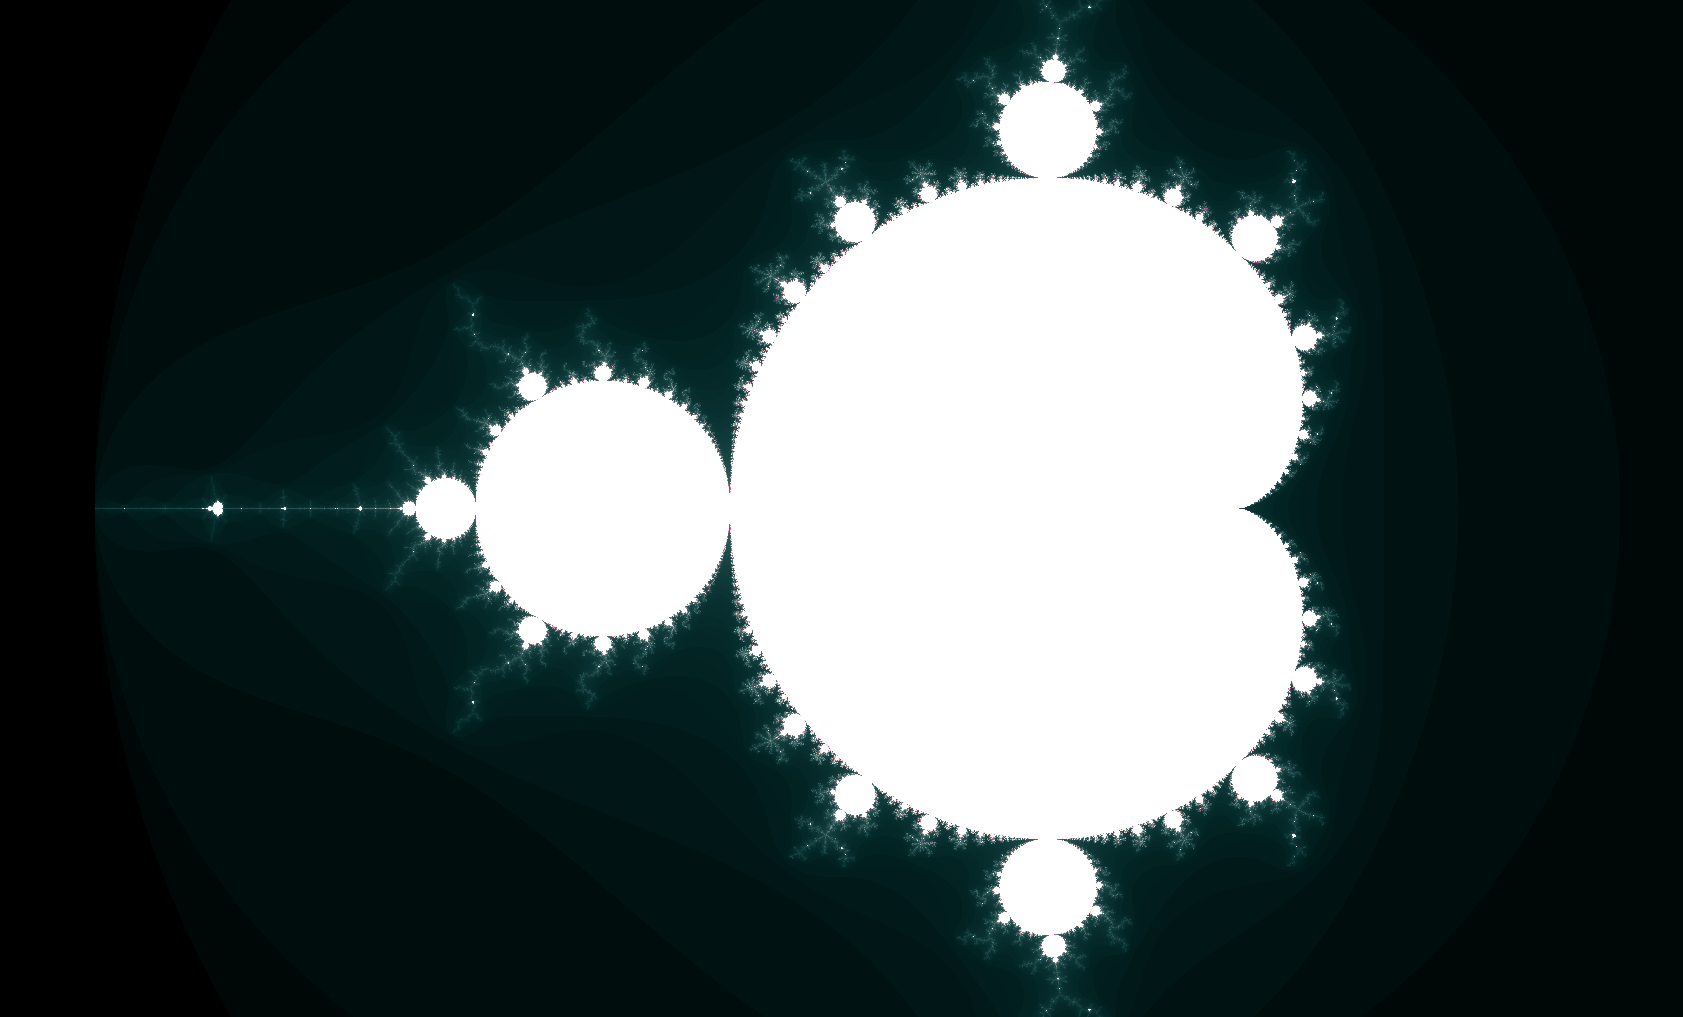
\includegraphics[width=0.65\linewidth, frame]{Images/Mandelbrot-2D-Full.png}
	\caption{The Mandelbrot set. The white points in the centre are inside the set.}
	\label{figure:mandelbrot-2d-full}
\end{figure}

The Mandelbrot set is the set of two-dimensional points that satisfy a certain constraint on the following complex quadratic equation:

\begin{equation} \label{equation:mandelbrot-2d}
	Z = {Z^2} + C
\end{equation}

where Z and C are complex numbers. The constraint on the points is that their orbit must be bounded. The value of Z is initialized to 0 and equation \ref{equation:mandelbrot-2d} is iterated over, each new value of Z being placed back in to the equation in the next iteration. If the length of the point Z does not exceed a threshold, then the point (represented by C) is in the Mandelbrot set \cite{devaney1999mandelbrot}.\newline

Figure \ref{figure:mandelbrot-2d-full} shows a generated Mandelbrot set. The real part of the point C is represented by the x-axis, and the imaginary part by the y-axis. Equation \ref{equation:mandelbrot-2d} is iterated over a maximum of five hundred times, and the threshold value is two. The pixels are coloured according to how many iterations are achieved before the length of Z exceeds the threshold.

\newpage

\begin{figure} [ht]
	\centering
	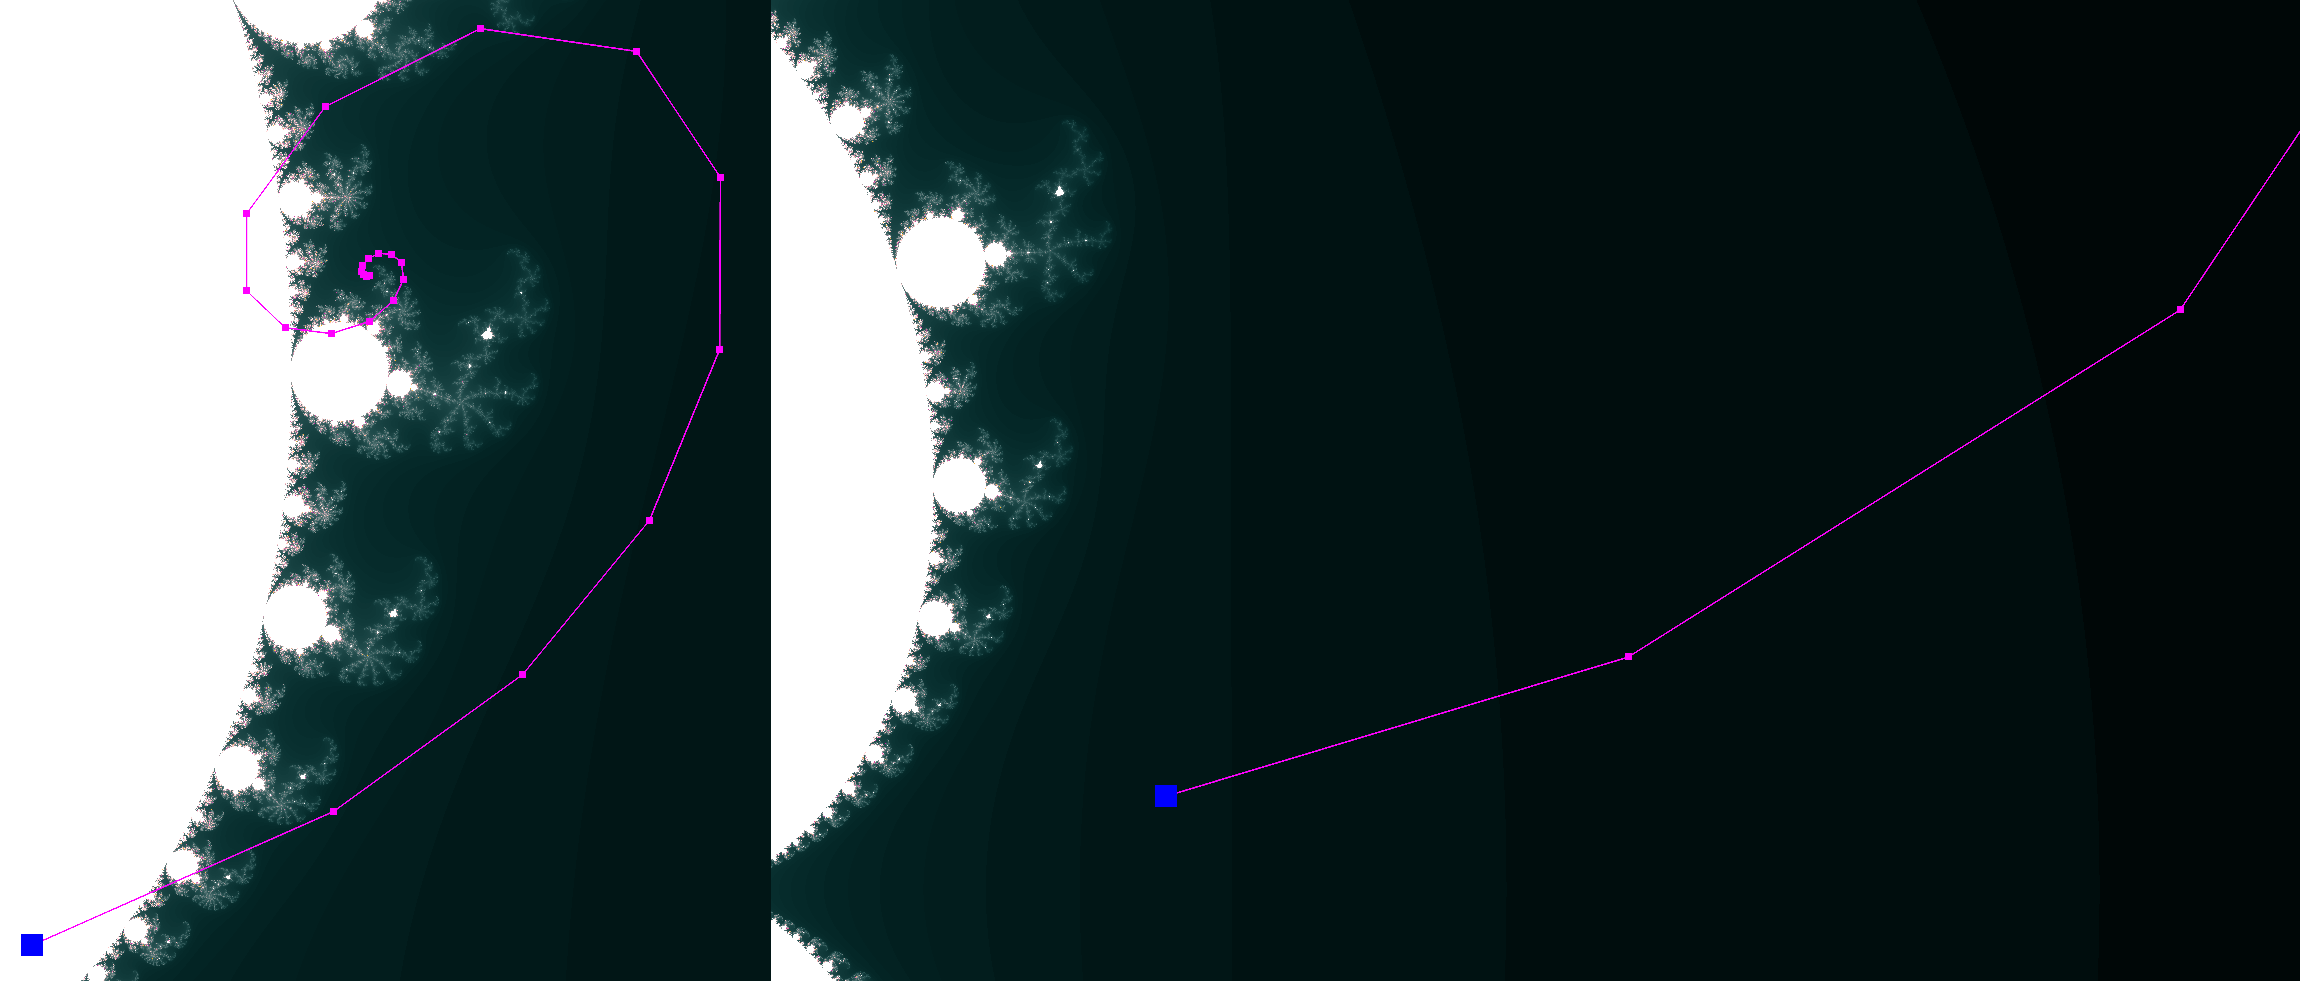
\includegraphics[width=\linewidth, frame]{Images/Mandelbrot-2D-Iterations.png}
	\caption{Visualization of the first twenty five iterations of equation \ref{equation:mandelbrot-2d} on the initial points [0.3, 0.05] (left) and [0.5, 0.04] (right). The initial points are shown in blue.}
	\label{figure:mandelbrot-2d-iterations}
\end{figure}

\begin{figure} [ht]
	\centering
	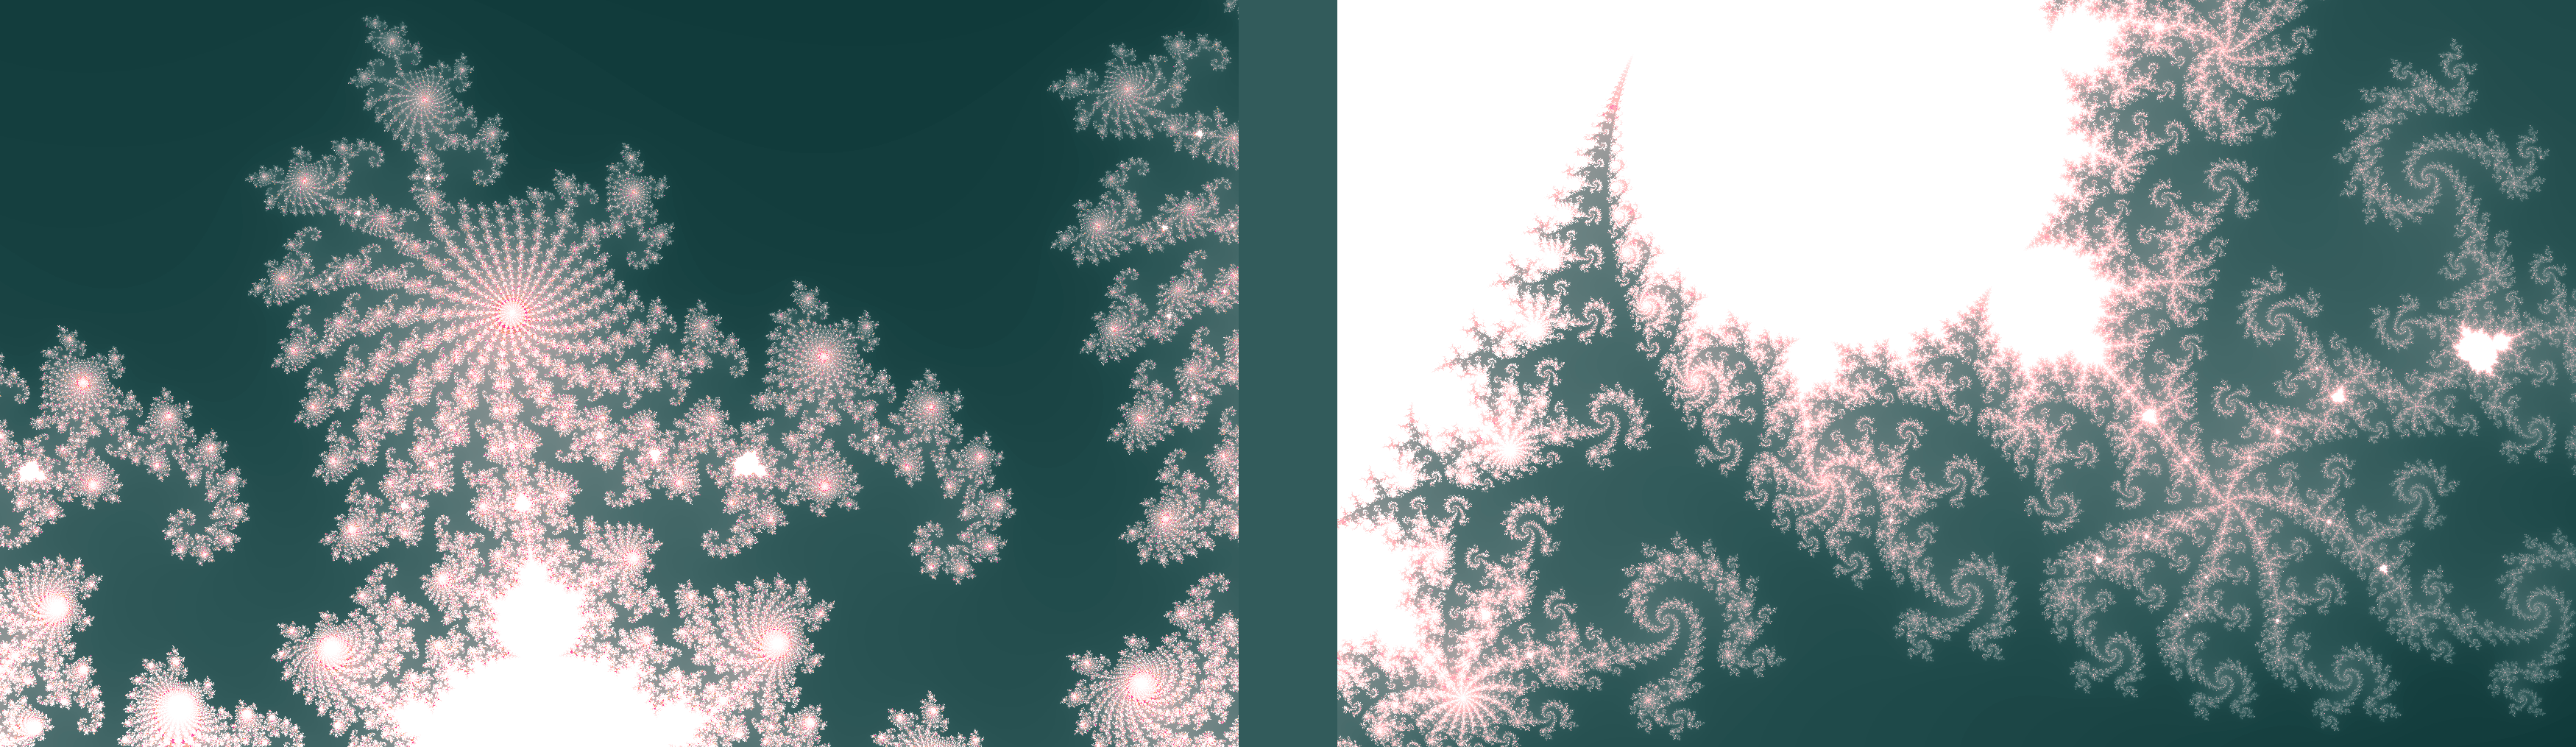
\includegraphics[width=\linewidth, frame]{Images/Mandelbrot-2D-Zoom.png}
	\caption{Two different views of the Mandelbrot set, zoomed in.}
	\label{figure:mandelbrot-2d-zoom}
\end{figure}

Figure \ref{figure:mandelbrot-2d-iterations} illustrates the first twenty five iterations on two different points. For the first point, the iterations converge in a spiral shape and the length of Z never exceeds the threshold of two, therefore the point is in the Mandelbrot set and is coloured white. For the second point, the iterations diverge and exceed the threshold of two within a few iterations, so this point is not in the Mandelbrot set and is coloured dark.\newline

Figure \ref{figure:mandelbrot-2d-zoom} shows two zoomed-in views at the edge of the original shape. New patterns can be seen, as well as repeated ones, and even new instances of the original shape. This is because the Mandelbrot set has infinite detail, so if one decreases the range of the axes, new patterns will emerge \cite{ashlock2006evolutionary}.\newline

This project makes use of three-dimensional fractal rendering, so the next section will look at the challenge of bringing this infinite level of detail to three dimensions.

\newpage

\section{3D Fractals - The Mandelbulb}

\begin{figure} [ht]
	\centering
	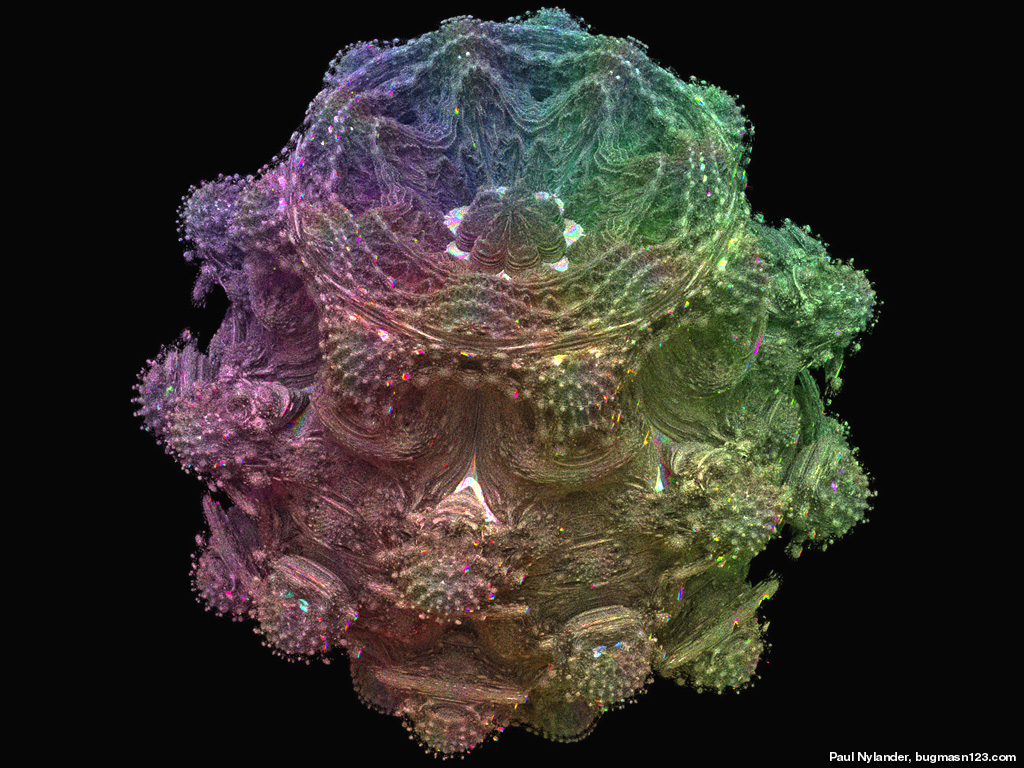
\includegraphics[width=0.5\linewidth, frame]{Images/Mandelbulb-First-Look.jpg}
	\caption{First look at the Mandelbulb, from Paul Nylander's website \cite{nylander-mandelbulb-image}.}
	\label{figure:mandelbulb-first-look}
\end{figure}

Since the Mandelbrot set is in two dimensions, and since complex numbers have only two components (real and imaginary), obtaining a true three-dimensional Mandelbrot set is a challenging task, and a mathematically rigorous three-dimensional Mandelbrot has not yet been found \cite{aron2009mandelbulb}.\newline

One attempt that seems to have come close was originated by Rudy Rucker in 1987. Rucker thought that expressing the three-dimensional points in spherical coordinates would allow the manipulation of the points in a similar way to the complex-number operations performed on the points in the two-dimensional Mandelbrot set \cite{rucker2009search}.\newline

Rucker did not have the computational power to accomplish a rendering of this idea, so it was put aside for twenty years, until Daniel White independently published a formula in 2007, which took the approach proposed by Rucker. White decided to approach the problem by considering the geometrical consequences of multiplying numbers in the complex plane, which amounts to rotating them \cite{aron2009mandelbulb}.\newline

White's formula produced images that looked promising, but they didn't have the level of detail that was expected from a true three-dimensional equivalent of the Mandelbrot set. A mathematician, Paul Nylander, raised White's formula to a higher power (eight), which would be equivalent to increasing the number of rotations of the point. The resulting image is shown in figure \ref{figure:mandelbulb-first-look}. The shape maintains excellent detail, even at high levels of magnification \cite {aron2009mandelbulb}.

\newpage

The new shape, known as the Mandelbulb, has roughly the same formula as the Mandelbrot set (equation \ref{equation:mandelbrot-2d}):

\begin{equation} \label{equation:mandelbulb}
	Z = {Z^k} + C
\end{equation}

where Z is raised to an arbitrary power like so:

\begin{equation} \label{equation:mandelbulb-power}
	{Z^k} = {r^k}(sin[k\theta]cos[k\phi], sin[k\theta]sin[k\phi], cos[k\theta]).
\end{equation}

The variable r is the norm of Z (|Z|), $\theta$ is equal to arctan($Z_y$/$Z_x$) and $\phi$ is equal to |($Z_x$, $Z_y$)|/$Z_z$. The spherical coordinates of the point Z/|Z| are represented by $\theta$ and $\phi$. Equations \ref{equation:mandelbulb} and \ref{equation:mandelbulb-power} are sourced from Chapter 33 of the book Ray Tracing Gems II \cite{marrs2021ray}.

\section{Signed Distance Functions}

Signed distance functions provide an estimate of how close a point is to the surface of a shape. If the result of the function is positive, then the point is outside the surface. If the result is negative, then the point is inside the surface. If the result is zero, then of course the point is exactly on the surface of the shape described by the function \cite{roblesprocedural}.\newline

A signed distance function can be derived using the B\"{o}ttcher map for the fractal formula, which is a deformation of the space. Closer to the surface of the fractal, the space is deformed to a greater degree than parts further away from the surface, as shown in figure \ref{figure:julia-bottcher-map}. The deformations of the space occur in such a way as to map the exterior of the fractal to the exterior of a unit disk \cite{quilez-distance}.\newline

A rigorous mathematical explanation of the B\"{o}ttcher map will not be given in this paper, but a brief introduction is helpful to understand the derivation of the distance function for the Mandelbulb. The map can be calculated as follows:

\begin{equation} \label{equation:bottcher-map}
	{\phi_C[Z]} = {lim_{n\rightarrow\infty}[f^n[Z]]^{k^{-n}}}
\end{equation}

where the value of f[Z] is the same as in equation \ref{equation:mandelbulb} and n refers to the current iteration of the equation \cite{marrs2021ray}.\newline

Looking at equation \ref{equation:bottcher-map}, take a point Z that is not in the fractal, so that the function f$^n$[Z] grows as the number of iterations increases, tending towards infinity. For a large enough value of n, the term f$_n$[Z] will become vastly larger than the value of C (as the point is far from the fractal), meaning that C can reasonably be discarded \cite{marrs2021ray}.

\newpage

\begin{figure} [ht]
	\centering
	
\includegraphics[width=0.5\linewidth, frame]{Images/Quilez-Bottcher-Map.jpg}
	\caption{The B\"{o}ttcher map generated for the Julia set (another two-dimensional complex fractal related to the Mandelbrot set), from the website of Inigo Quilez \cite{quilez-distance}.}
	\label{figure:julia-bottcher-map}
\end{figure}

From this casting away of C we obtain:

\begin{equation} \label{equation:mandelbulb-without-c}
	{f^{n+1}[Z] \approx {(f^n[Z])^k}}
\end{equation}

for points that are sufficiently far away from the surface of the fractal. Since the point at iteration n is far from the fractal, if one were to undo all of the iterations to get back to the original point at f$_0$[Z], we would obtain this expression:

\begin{equation} \label{equation:reverse-iterations}
	{{f_0^{n}[Z]}^{k^{-n}}} = Z
\end{equation}

and by extension, returning to the B\"{o}ttcher map:

\begin{equation} \label{equation:reverse-iterations-bottcher}
	\phi_0[Z] = Z
\end{equation}

which is the approximate result that equation \ref{equation:bottcher-map} gives when the function f$^n$[Z] ultimately diverges \cite{marrs2021ray}.\newline

Next, we will use something called the Hubbard-Douady potential, equal to the logarithm of the modulo of the B\"{o}ttcher map. This is a map of points onto a unit disk. Recall that the B\"{o}ttcher map maps the exterior of the fractal to the exterior of a unit disk. This now becomes important, as it enables us to use the Hubbard-Douady potential for all of our complex fractals. We now have a function that tends towards zero as the points approach the boundary of the fractal \cite{quilez-distance}:

\begin{equation} \label{equation:hubbard-douady}
	G[Z] = {lim_{n\rightarrow\infty}}\frac{log|{f^n}[Z]|}{k^n}.
\end{equation}

Equation \ref{equation:hubbard-douady} is not ready to be used as a distance measurement yet. However, it's possible to make it so. More detail is given in Ray Tracing Gems II, but a brief explanation will be given here. If we divide G[Z] by its gradient (obtaining this from the first-order Taylor expansion of the function), then we obtain an upper bound on the distance to the surface, which is desirable. The final equation for distance estimation therefore is \cite{marrs2021ray}:

\begin{equation} \label{equation:final-distance-estimate}
	d(Z) = {lim_{n\rightarrow\infty}}\frac{|f^n(Z)|log|f^n(Z)|}{|(f^n)'(Z)|}.
\end{equation}

\section{Ray and Sphere Tracing}

Ray tracing is a technique used for rendering scenes. Generally, a ray is a line that is cast from the camera or eye through each pixel of an image. Tests are performed to see which object (if any) is encountered by the ray first. By bouncing the ray from object to object, the program can gather the various light contributions from objects that reflect, emit or refract light \cite{haines2019ray}.\newline

Distance estimators can be used for ray tracing. If the approximate distance to the nearest surface can be calculated then the current point can be moved along the ray safely, until it is close enough to the surface to stop, according to this formula:

\begin{equation} \label{equation:sphere-tracing}
	{P_{n+1}} = {P_n} + \textbf{v}d({P_n})
\end{equation}

where P$_{n+1}$ is the point at the next step, P$_n$ is the point at the current step, \textbf{v} is the unit vector representing the ray direction and d(P$_n$) is the distance function acting on the current point \cite{marrs2021ray}.\newline

Using a distance function in this way is known as sphere tracing. The magnitude of the result of the distance function can be considered as the radius of a sphere. This sphere is guaranteed not to go through any part of the surface, making it safe to step according to the distance function result in any direction. For this guarantee to hold, the distance function must either be an exact calculation of the distance, or an underestimate \cite{hart1996sphere}.\newline

See figure \ref{figure:sphere-tracing}. This shows three scenarios for tracing a ray with the sphere tracing technique. At the bottom, the distance function is an exact measure of the distance to the nearest point on the surface. This is the ideal scenario, for correctness and performance. The top left image shows the result of a distance function which underestimates the distance each time. As a result, significantly more steps are taken along the ray, which will result in decreased performance. Lastly, the top right image shows the result of overestimating the distance. The ray ends up stepping past the boundary of the shape.

\newpage

\begin{figure} [ht]
	\centering
	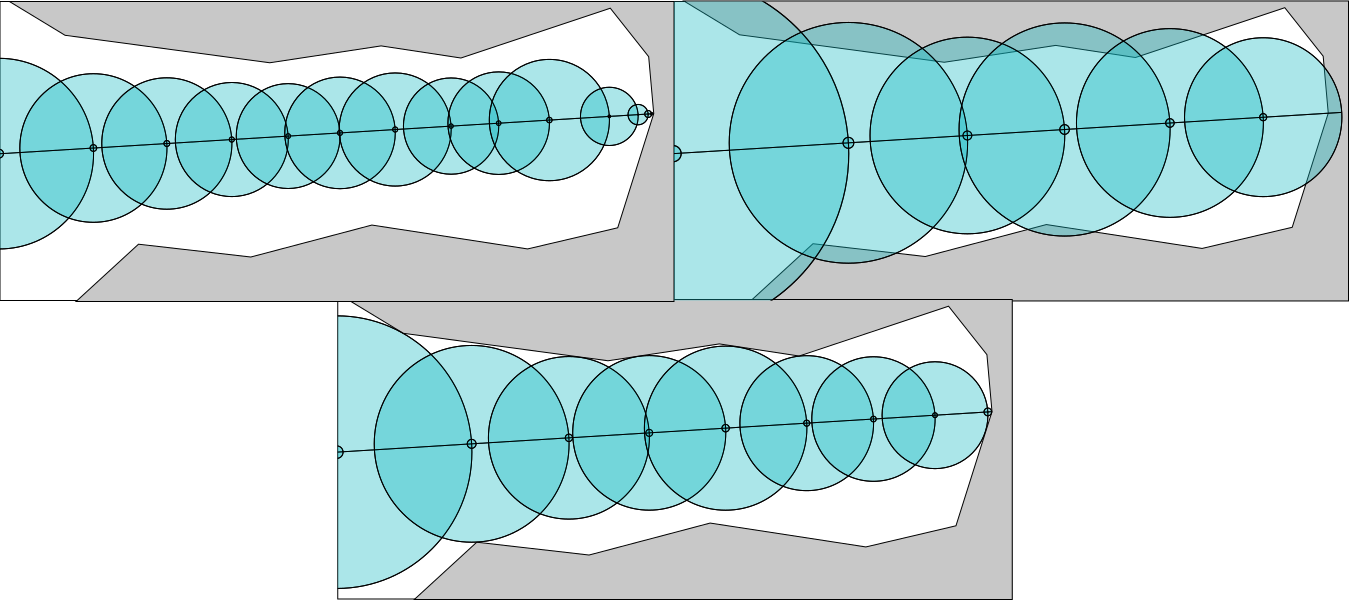
\includegraphics[width=0.75\linewidth, frame]{Images/Sphere-Tracing.png}
	\caption{Three scenarios in sphere tracing. Top left: Distance function underestimates distance, resulting in a loss of performance. Top right: Distance function overestimates distance, resulting in a loss of accuracy. Bottom: Distance function is exact.}
	\label{figure:sphere-tracing}
\end{figure}

\section{Signed Distance Fields}



Papers:
\begin{itemize}
	\item Signed distance fields: A natural representation for both mapping and planning \cite{oleynikova2016signed}.
	\item Hierarchical hp-adaptive signed distance fields \cite{koschier2016hierarchical}.
	\item Interactive ray tracing of distance fields (page 91) \cite{jamrivska2010interactive}.
\end{itemize}

- Stored values from signed distance function, stored as 2D texture or 3D grid.

- Saves having to recompute SDF all the time.

- Fractal scenes with high view distance could benefit from some pre-calculated values to give them a head start - show room of pillars and remark on frame rate (no SDF).

- Remark on memory costs.

- Briefly talk about storage methods - octrees.

- Talk about 2D methods - particularly used for fonts.

\section{Temporal Caching} \label{section:temporal-caching}
\chapter{System Design}
\label{chapter:system-design}

This chapter will go through the design of the project software. First, the system requirements will be laid out, followed by the general system design. The system design is simple, as the focus is on improving the performance of rendering.

\section{System Requirements}

\subsection{Functional Requirements}

\begin{itemize}
	\item The software will use fragment shaders to render 3D fractals using sphere tracing.
	\item The software will provide user controls for camera motion.
	\item The software will implement a Signed Distance Field for optimization.
	\item The software will implement a temporal cache for optimization.
	\item The software will be capable of measuring the performance of the rendering process.
	\item The software will be capable of writing these measurements to file in an easily readable format.
	\item The software will be configurable through program arguments.
\end{itemize}

\subsection{Non-Functional Requirements}

\begin{itemize}
	\item The software should be easy to use, with helpful instructions in the README file and printed to the terminal on load.
	\item The software user controls should be intuitive.
	\item The software arguments should be clearly explained.
	\item The software should be stable (it should not crash or have obvious bugs).
	\item The software should have a sensible layout in the code repository.
\end{itemize}

\section{System Design}

The project must include several components. One of these is a renderer, capable of rendering 3D fractals to the screen. This must be configurable through the program's arguments, as the different optimization methods will have different requirements. The next component is the implementation of the two optimization techniques. These will affect the configuration of the renderer as well. Lastly, performance measurements must be taken. These should not affect the rendering process.\newline

With these components, the overall system design is simple. There is no GUI to implement, so no overall design or consideration for the user experience. The main design consideration is in the configuration of the various states of the program. A design for the arguments that the program will take, and how they will affect the program at run time, is considered now.

\subsection{Program Arguments}

The various configurations of the system at run time will be decided via the program's arguments. These will be as follows:\newline

The plan is to render more than one type of fractal, so these will need to be selected via the first argument. The type of fractal affects which signed distance function to use, so is needed to select the shaders to load.\newline

The focus of the project is the improvement of performance, so the various methods will need to be compared to each other. The second input to the program will decide which optimization method to use; in this case, the options are no optimization, the SDF and the temporal cache. This will further affect which shaders will get loaded, as well as some other settings in the renderer.\newline

A real time rendering project would not be very useful if it did not allow animation or movement of some kind. With that in mind, it might be of interest to see how the different optimization methods perform when running animations. The third argument will select whether to animate the scene. This will not affect which shaders are loaded, only which data is passed into them.\newline

The last arguments control the measurement of performance. Argument 4 will control whether performance measurements are taken at all, and argument 5 will contain the name of the file to be written out to. Data will be written to the file specified in a readable format.
\chapter{Implementation}
\label{chapter:implementation}

This chapter will go through the implementation of the project software. First, the system information and general program structure will be looked at. Then, the rendering of fractals will be covered, followed by the attempts at improving performance, and the method of measuring performance. Finally, there will be a section on debugging.\newline

In terms of general optimizations, there were no specific efforts to optimize the code or the basic algorithms (except perhaps to implement a view distance limit), since the most important thing was to remain consistent across the different scenarios, and the relevant measurements were the performance differences (if any), not the raw performance.

\section{Operating System and Hardware}

The operating system used was Linux Mint 20.1. No other operating system was tested.\newline

The CPU used was an Intel\copyright Core$^{TM}$ i7-9750H with 6 cores.

The GPU used was an NVIDIA TU106M (GeForce RTX 2060 Mobile).

The Vulkan version being used was 1.3.205.

\section{Program Structure and Libraries}

\subsection{Build System}

The build system chosen was Make. The project is small in terms of the code base so writing a Makefile for compilation was simple. A shell script was also written, and run from Make, that used GLSLC to compile the shaders and place them in the appropriate directories. GLSLC is licensed under the Apache License Version 2.0 \cite{licensing-glslc}.

\subsection{Language and Libraries Used}

The programming language of choice for this project was C, because it is the language that the libraries used were written in, and it's simple and efficient.

\subsubsection{Vulkan}

Vulkan was chosen because it is performant and modern, and because there is a new feature on the way that will, I think, help with the efficiency of rendering using one of the optimization methods chosen (this will be mentioned in the Conclusion chapter). It is licensed under the Apache License 2.0 \cite{licensing-vulkan}.

\subsubsection{Volk}

The third-party library, Volk, is a meta-loader for Vulkan. It allows one to load the Vulkan API without needing to link to Vulkan. This makes setup much easier to manage. It is licensed under the MIT license \cite{licensing-volk}.

\subsubsection{GLFW}

GLFW is a library for creating windows and surfaces, which can be used for Vulkan development. Additionally, it is easy to use and multi-platform, so was the logical choice for this project. It is licensed under the zlib/libpng license \cite{licensing-glfw}.

\subsection{Vulkan Setup}

The rendering process was split into two passes, one for geometry and one for colour. This was done because the speed at which the geometry of the scene was obtained was of interest, and the speed of colouring the fractals was not, so splitting them enabled measurement of the geometry render pass on its own. No vertices are passed in to the shaders; the vertex shaders conjure up fullscreen triangles using the vertex indices, which are then worked on by the fragment shaders, where all the calculations and colouring happen.\newline

Specific setups for different optimization methods will be discussed in the relevant sections.

\subsection{Program Arguments and Controls}

The program takes arguments which specify the setup when the program is loaded. The user can change which fractal to display (including the 2D Mandelbrot set, the Mandelbulb and the Hall of Pillars), which optimization method to use, whether to vary any fractal parameters (which can be used to animate the fractal) and whether to take any performance measurements during runtime. Some of the arguments affect which shaders are loaded, and the Vulkan setup.\newline

The user is able to control the camera with the mouse and keyboard, speed up and slow down, and print the current position and camera front vector. Input is handled by GLFW.

\section{Rendering 3D Fractals}

The project made use of two fractal formulae. One was for the Mandelbulb, as described in the background section. Another was chosen to provide variety, specifically with regards to the depth of the image. The Mandelbulb is neatly contained within a box, and the program renders its exterior, but not any `interior'. The alternative fractal (named `Hall of Pillars' by me given its lack of another name) is reminiscent of a room with many archways, which I thought might give a greater variety of results in terms of the performance measurements when using the optimizations developed in the project.\newline

The calculations for the fractals were done entirely within shaders, except for the generation of the 3D signed distance field, which was calculated on the CPU upon loading the program, before any rendering occurred. Single-precision floating point numbers were used for all calculations within shaders. These were chosen over double-precision numbers, as the scale of the fractals was reasonable, and high-detail zooms into the fractal were not necessary for the project.

\subsection{Basic Sphere Tracing Implementation}

The basic sphere tracing algorithm was implemented in GLSL and is largely the same across the fractal types and optimization methods. Figure \ref{figure:glsl-sphere-tracing} shows the implementation.

\begin{figure}[ht]
	\centering
	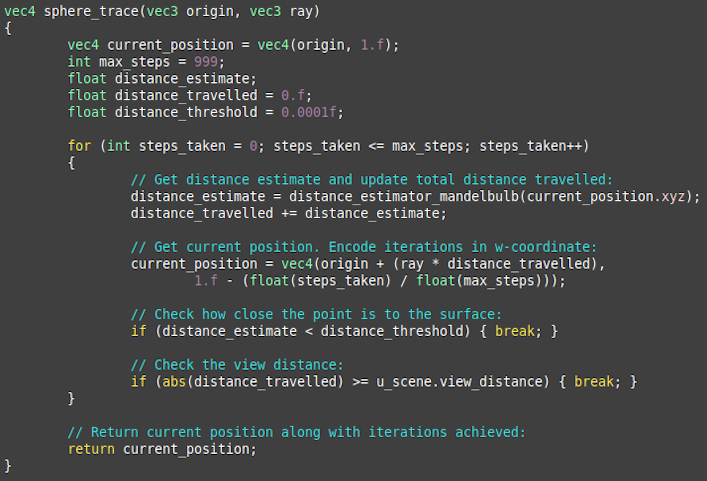
\includegraphics[width=0.65\linewidth, frame]{Images/GLSL-Sphere-Tracing.png}
	\caption{GLSL code snippet of the sphere tracing algorithm.}
	\label{figure:glsl-sphere-tracing}
\end{figure}

The most important things that must remain consistent between different optimizations on the same fractal are the termination conditions, which are as follows:

\begin{itemize}
	\item The maximum number of iterations allowed.
	\item The distance threshold.
	\item The view distance, contained in the scene uniform.
\end{itemize}

\subsection{Mandelbulb Fractal}

\begin{figure}[ht]
	\centering
	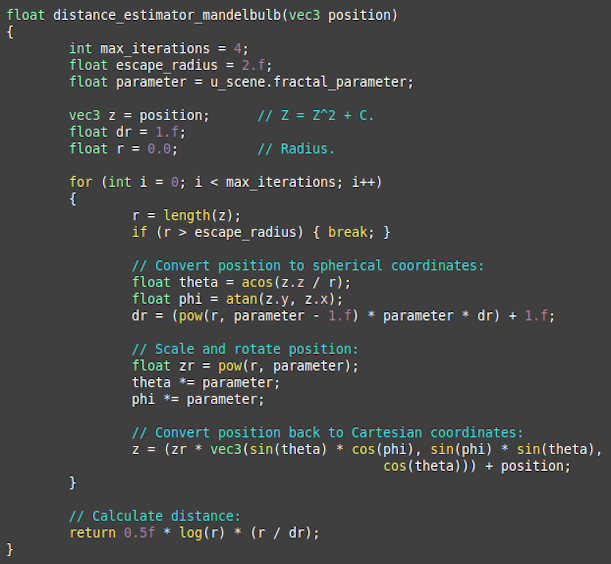
\includegraphics[width=0.65\linewidth, frame]{Images/GLSL-Distance-Estimator-Mandelbulb.png}
	\caption{GLSL code snippet of the distance estimator function for the Mandelbulb fractal.}
	\label{figure:glsl-distance-estimator-mandelbulb}
\end{figure}

\begin{figure}[ht]
	\centering
	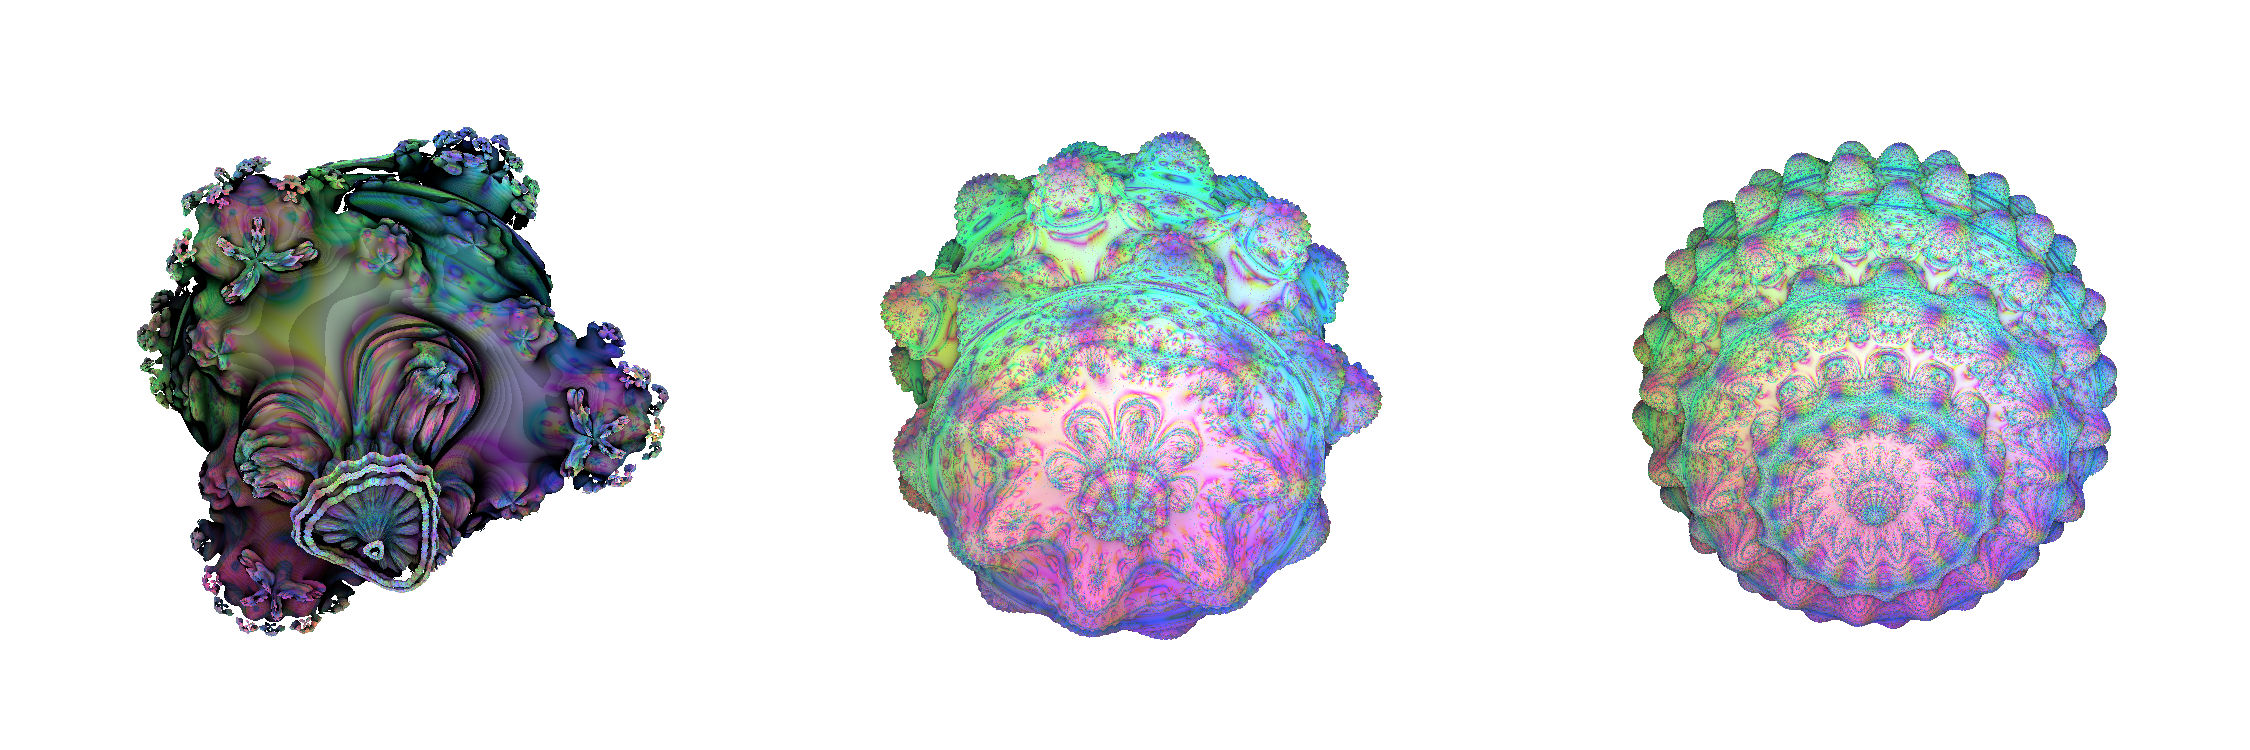
\includegraphics[width=0.65\linewidth, frame]{Images/Mandelbulb-Powers.png}
	\caption{The Mandelbulb, raised to different powers. Left to right: four, eight, sixteen.}
	\label{figure:mandelbulb-powers}
\end{figure}

Figure \ref{figure:glsl-distance-estimator-mandelbulb} shows the implementation of the distance estimator for the Mandelbulb fractal. Recall equations \ref{equation:mandelbulb} and \ref{equation:mandelbulb-power}. Equation \ref{equation:mandelbulb} is iterated over four times maximum. During the iterations, the current point is converted to spherical coordinates, scaled, and then converted back to Cartesian coordinates using equation \ref{equation:mandelbulb-power}. The distance formula based on equation \ref{equation:final-distance-estimate} is used to get the final result. The gradient of |f(Z)| is computed during the iterations (represented by dr in the shader).\newline

The fractal parameter in the scene uniform is the power that Z is raised to in the Mandelbulb formula. Varying this parameter results in different forms of the Mandelbulb. By default this parameter is eight, to match the original discovery by Paul Nylander. Figure \ref{figure:mandelbulb-powers} illustrates the effect of varying this parameter.

\subsection{Alternative Fractal}

\begin{figure}[ht]
	\centering
	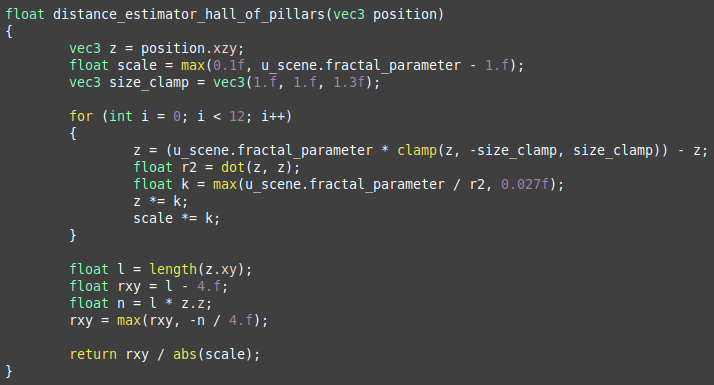
\includegraphics[width=0.65\linewidth, frame]{Images/GLSL-Distance-Estimator-Hall-Of-Pillars.png}
	\caption{GLSL code snippet of the distance estimator function for the Hall of Pillars fractal. Full credit goes to Dave Hoskins for the formula \cite{shadertoy-hall-of-pillars}.}
	\label{figure:glsl-distance-estimator-hall-of-pillars}
\end{figure}

\begin{figure}[ht]
	\centering
	
\includegraphics[width=0.65\linewidth, frame]{Images/Hall-Of-Pillars-Example.png}
	\caption{Rendering of the Hall of Pillars fractal.}
	\label{figure:hall-of-pillars-example}
\end{figure}

Figure \ref{figure:glsl-distance-estimator-hall-of-pillars} shows the implementation of the distance estimator for the alternative `Hall of Pillars' fractal. This fractal has different mathematical origins to the Mandelbulb, and is known as a Pseudo Kleinian fractal, but the mathematical background will not be explored here \cite{pseudo-kleinian-fractals}.\newline

As you can see from figure \ref{figure:hall-of-pillars-example}, this fractal varies a lot in depth, and  in particular has a lot of holes in it, so will result in the bottlenecks discussed in section \ref{section:temporal-caching}. The fractal formula was chosen for this reason, and to give variety when collecting results. Exploring the fractal also reveals large flat sections, and even larger `halls' much like the one in figure \ref{figure:hall-of-pillars-example}, as well as more intricate sections with great depth variety, but less overall depth. This fractal provided a good set of representative views for results collection.

\subsection{Colour}

Colour was not of the utmost importance in the project, so this section will be very brief. Colouring of the mandelbulb was done based on the closest distance from each point in the image to some fixed point. The Mandelbulb equation was iterated through, as in the distance estimation function, but in each iteration, the distance of the current point to a fixed point was measured, and the minimum of these was taken as a colour value.\newline

For the Hall of Pillars fractal, the colour was obtained in each iteration by getting the difference between elements of the current point and the previous point, and accumulating these differences.

\subsection{Ambient Occlusion}

\begin{figure}[ht]
	\centering
	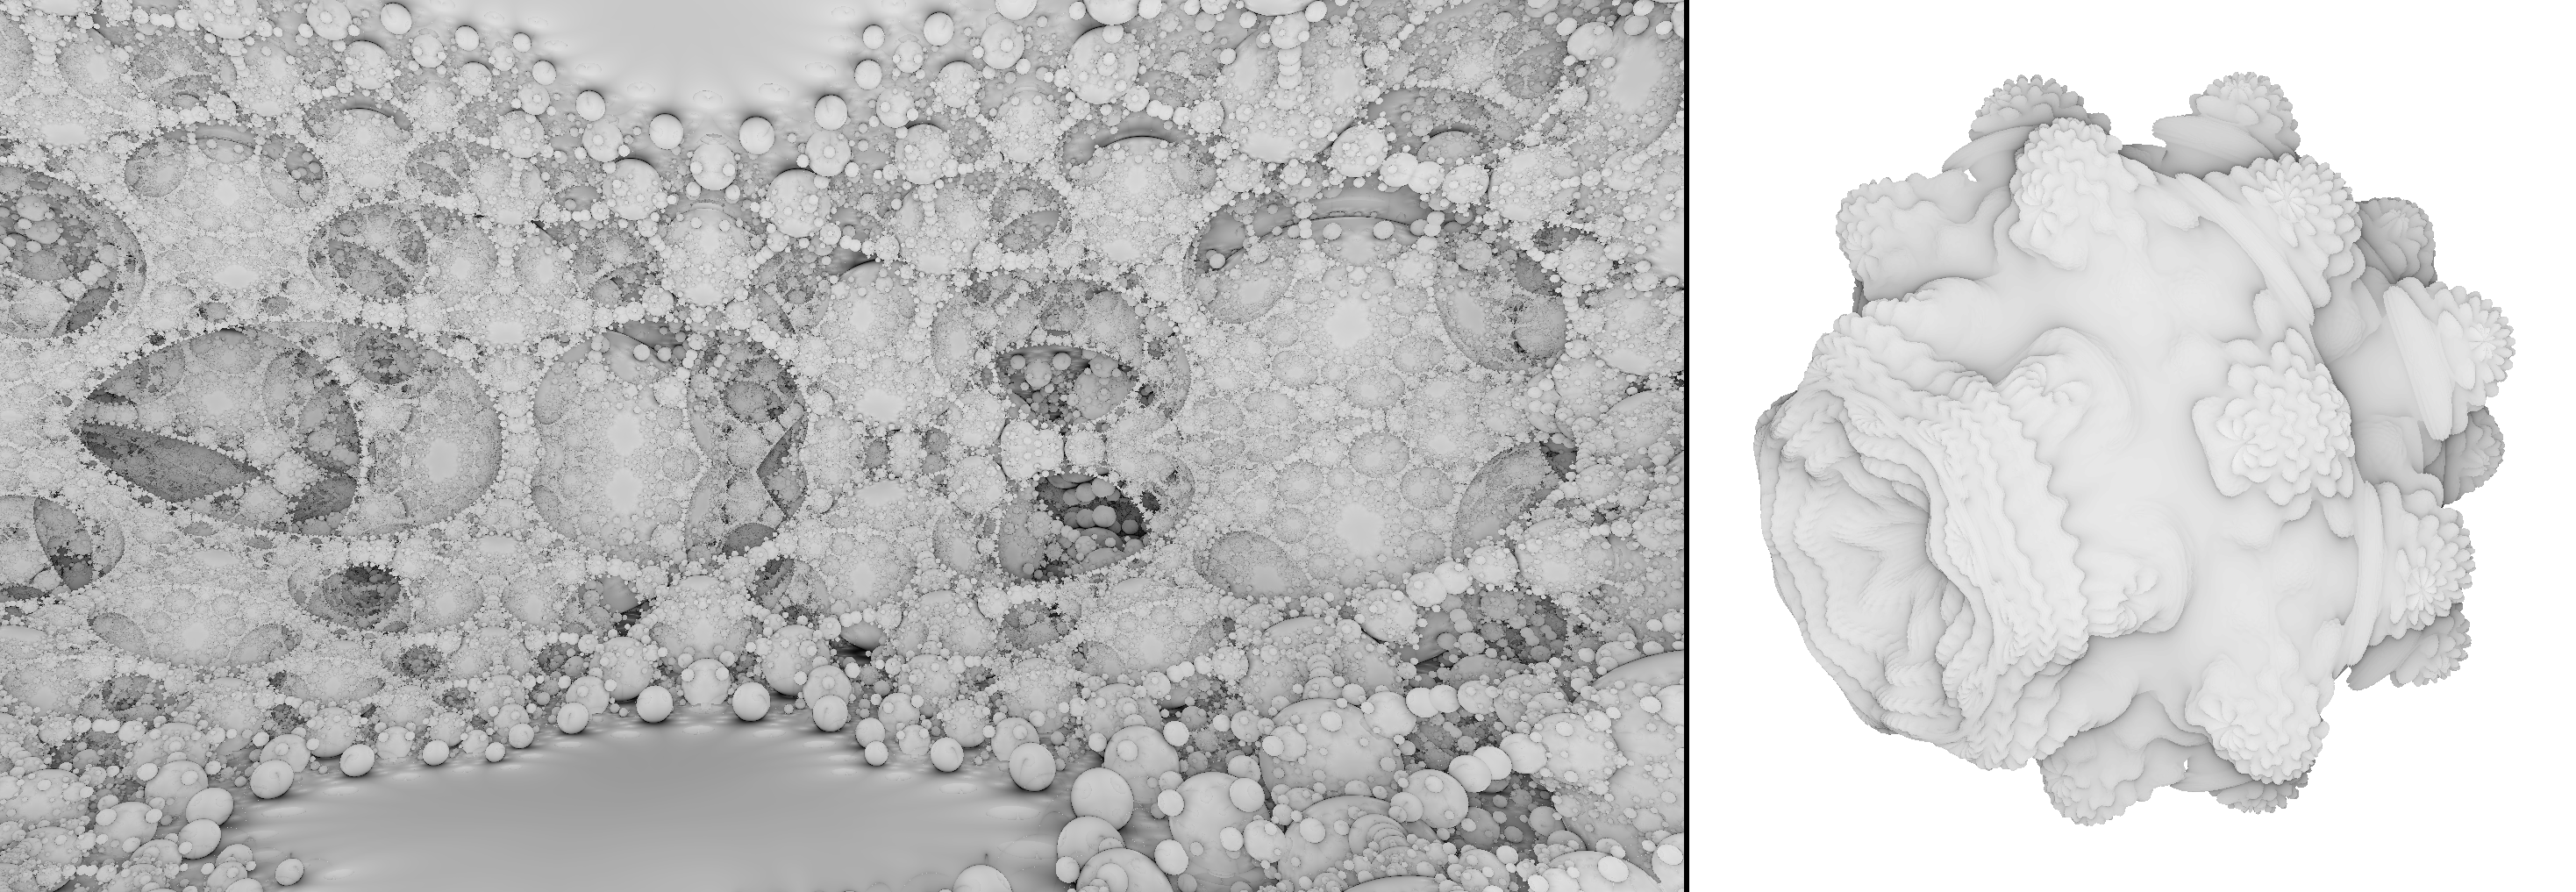
\includegraphics[width=\linewidth, frame]{Images/Ambient-Occlusion.png}
	\caption{Rendering of the Hall of Pillars fractal (left) and Mandelbulb (right), coloured based on the number of iterations achieved before reaching the surface.}
	\label{figure:ambient-occlusion}
\end{figure}

One of the consequences of using sphere tracing of signed distance functions is that it gives an estimate of the complexity of the surface. If a point takes more iterations to reach, then it's likely in a more complex area, and will be occluded. For both fractals in the project, the final colour is multiplied by a value between zero and one, based on the number of iterations achieved before reaching the surface. Figure \ref{figure:ambient-occlusion} shows renderings of the fractals used in this project, coloured purely based on the number of iterations.\newline

This free ambient occlusion effect also gives an informal measure of performance. Brighter areas mean less iterations, so two identical views can be compared which are using different optimization methods, to see if one performs better in terms of the number of iterations. Since this was the aim of using temporal caching, this was used as a measure of performance, in addition to render pass timings.

\section{3D Signed Distance Field}

\begin{figure}[ht]
	\centering
	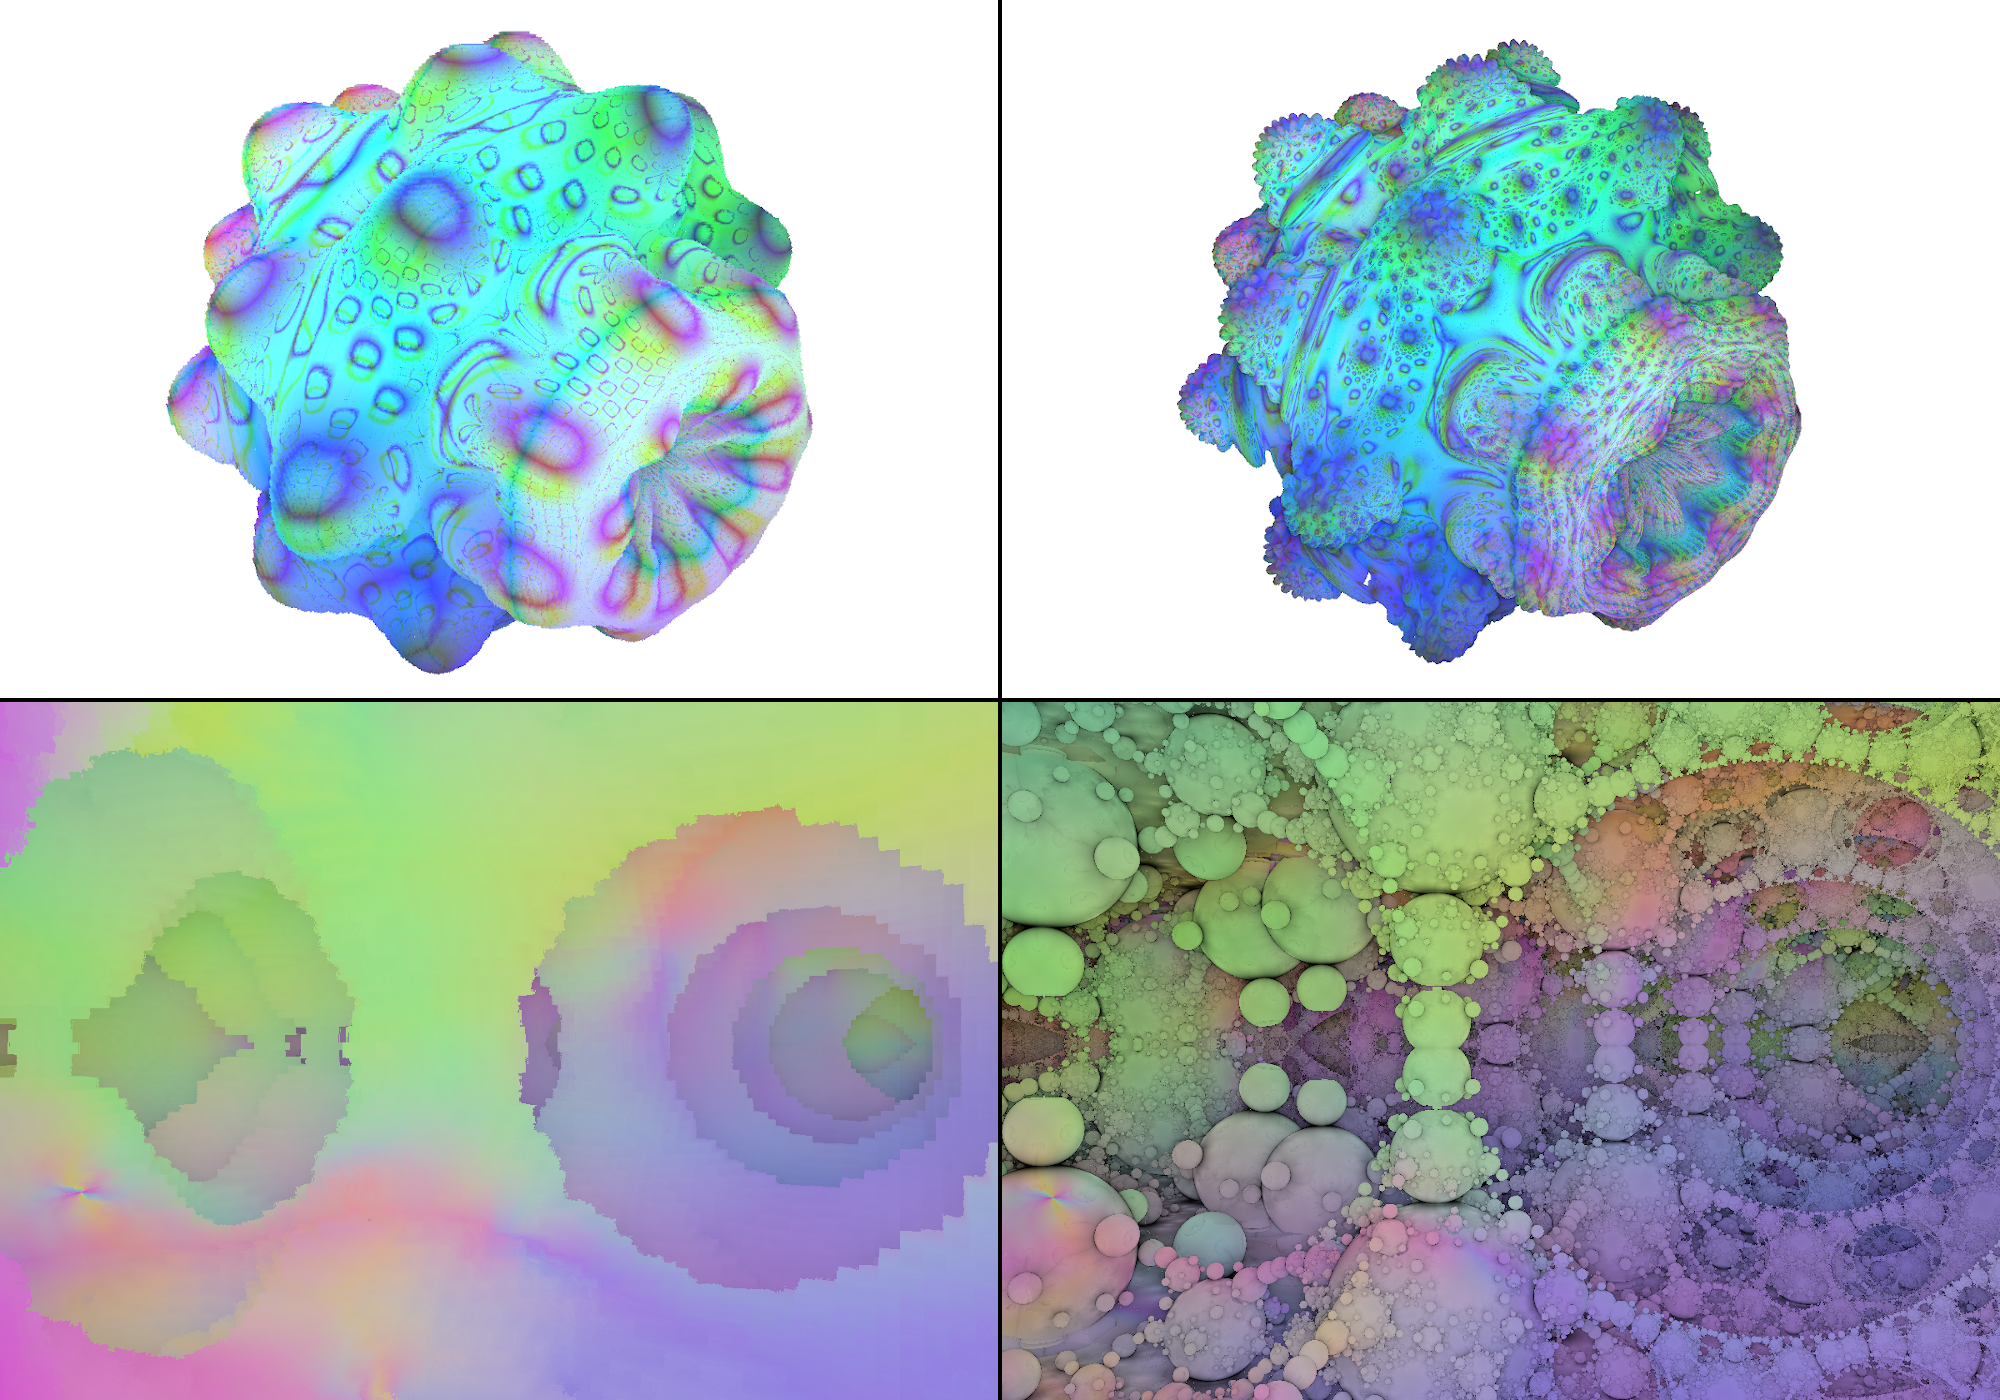
\includegraphics[width=0.65\linewidth, frame]{Images/SDF-Hybrid-Comparison.png}
	\caption{Rendering of the Mandelbulb (top) and Hall of Pillars fractal (bottom), using the signed distance field alone (left) and the hybrid approach (right). The Mandelbulb is rendered with 8 levels of subdivision (256$^3$ voxels), and the Hall of Pillars is rendered with 9 levels (512$^3$ voxels).}
	\label{figure:sdf-hybrid-comparison}
\end{figure}

\subsection{Structure and Usage}

The signed distance field represented a three-dimensional grid. Samples were taken at the centre of each voxel in the grid. To obtain a guaranteed underestimate here, the length of the line between the centre and corner of the voxel was taken away from this distance (or added, if the distance was negative). The more common approach is to sample the distance at the corners of the voxels and interpolate based on the location inside. The decision to only take the centre value was made to reduce memory reads, as the signed distance functions for the fractals are cheap in comparison to, say, the signed distance function for an arbitrary polyhedral shape.\newline

Another design decision that was made was to take a hybrid approach. Rather than try to obtain as much detail as possible (and use a lot of memory) in the signed distance field, the program performed sphere tracing through the field, until the sampled distance was smaller than the size of the diagonal between the voxel centre and corner; the largest distance possible from the centre before leaving the voxel. Obtaining a value such as this means that the surface is likely within the voxel. When this happens, the program reverts to using the signed distance function to obtain the finer detail. This provides a balance between speed, memory use and accuracy. Figure \ref{figure:sdf-hybrid-comparison} shows a comparison of visual quality for both fractals used in the project when using a signed distance field with the signed distance field alone, and using the hybrid approach.\newline

For the Hall of Pillars fractal particularly, the signed distance field does not have nearly the required level of detail, despite it having one more level of subdivision than the Mandelbulb. This is because this fractal has a much larger scale, so in order to cover a reasonable area of the fractal with the field, each voxel must be much larger. For the Mandelbulb, the whole shape can be contained in a small box, approximately 2.2 units along each edge. The Hall of Pillars fractal seems to be infinitely large. This difference makes the signed distance field very limited for use in large fractals.

\subsection{Octree Storage}

\begin{figure}[ht]
	\centering
	
\includegraphics[width=0.4\linewidth, frame]{Images/Octree-Structure.png}
	\caption{Structure of the SDF octree. Only children of traversed nodes are shown.}
	\label{figure:octree-structure}
\end{figure}

\begin{figure}[ht]
	\centering
	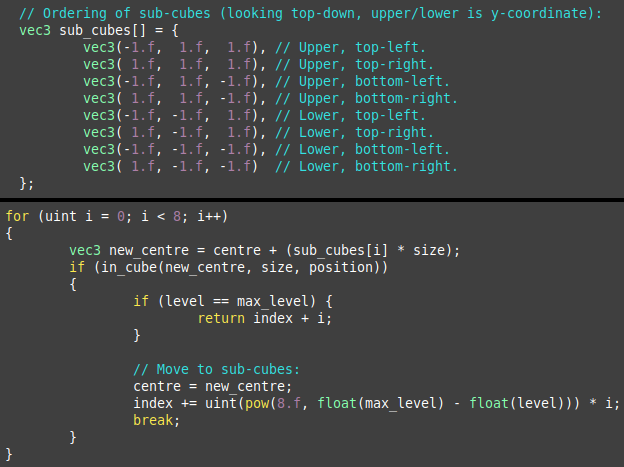
\includegraphics[width=0.55\linewidth, frame]{Images/Octree-Traversal.png}
	\caption{Code snippets from the octree traversal function. The voxel index is incremented by the number of leaf nodes that must appear when traversing the entire tree that comes before the current node.}
	\label{figure:octree-traversal}
\end{figure}

The signed distance field is represented as an octree. Figure \ref{figure:octree-structure} shows the layout. Only the leaf nodes hold data, and the higher level nodes aren't represented at all. The decision was made not to adaptively subdivide the tree to make a sparse layout. This is because it was desirable to reduce the number of memory reads, and instead calculate the index of the desired voxel by its depth and position inside the bottom level of the tree. This ruled out the use of adaptive sparse structures, as they would require more information on the subdivision of voxels, and so need to store information for higher-level voxels.\newline

The child nodes of every parent node are stored in the same order, which is what makes it possible to calculate the index without explicitly storing information about non-leaf voxels. In memory, the whole structure is represented as an array of floating point numbers; the calculated distances at the centre of each voxel. Additional, vital information is given in the scene uniform. This includes the size and centre of the root voxel, and the total number of subdivisions of the signed distance field. The values in the array are ordered left to right, as the leaf nodes would be if the whole tree was expanded.\newline

Figure \ref{figure:octree-traversal} shows a snippet of shader code for traversing the tree. No memory reads are required until the index of the leaf voxel is found (this function returns said index, which is used to fetch the data in the main sphere tracing function), so most of the effort is spent traversing the tree and calculating the index. This is in line with the goal of introducing as few memory reads as possible, since they are comparatively slow. As mentioned, for an arbitrary, complex polyhedral shape, this might not be a problem, but the fractals are fairly efficient to calculate, so the signed distance field traversal needs to be competitive.\newline

The calculation of the voxel index is based on its current level in the tree, compared to the maximum level, and its current position in the group of eight child voxels (see the lower image in figure \ref{figure:octree-traversal}). The centre positions of each voxel are calculated based on the position in the group of child voxels (the index of the loop is used to get a value from the array of positions, seen in the top of figure \ref{figure:octree-traversal}), and the current voxel size, which begins equal to the total signed distance field size, and is halved upon entering each new level.

\section{Temporal Caching}

\subsection{Data to Cache}

The data chosen to persist across frames was the true distance travelled by the ray. The aim of this optimization method was to reduce the number of iterations in certain areas of the image, especially edges and holes, so just storing the first distance estimate was not the solution. In order to preserve depth data for multiple frames, a texture image with red, green, blue and alpha floating-point components was chosen. With this, the data for the last four frames was stored. The reasoning behind only using one texture image was that sampling a texture requires an overhead that quickly builds up, so storing too much data may offset any performance benefit.

\subsection{Image Sampling}

The distance values were written to the G-Buffer for the first render pass. Every frame, the values were shifted one place to the right, discarding the last (alpha) value each time, and the new value was written to the first slot. After the render pass, the G-Buffer image was the copied over to a texture image, ready for sampling from during the next frame. Each pixel only sampled from its own position in the texture. It could be possible to do a kind of edge detection based on the depth values in neighbouring pixels, but this was deemed too expensive.

\subsection{Camera Movement}

\begin{figure}[ht]
	\centering
	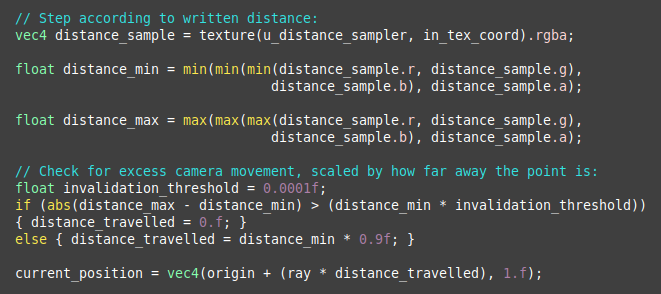
\includegraphics[width=0.65\linewidth, frame]{Images/Distance-Test.png}
	\caption{Test to determine if a pixel is invalid and the ray needs recasting.}
	\label{figure:distance-test}
\end{figure}

The test to see if the camera had moved too much is shown in figure \ref{figure:distance-test}. It relied on the difference between the largest distance sample and the smallest. Generally speaking, the `landscape' of the fractals chosen is not smooth, so this proved to be a reliable test for invalidated geometry, without triggering at the smallest movement. If the test passed, and the pixel was still valid, the minimum sampled distance estimate was chosen and reduced a little, to provide a reliable underestimate of the true distance for the current frame. The usual sphere tracing algorithm was then performed, using this head-start.\newline

Alternative data for testing for camera movement was considered as well, such as end position, end distance estimate and the lowest distance estimate along the ray, but in the end, storing the true distance travelled for the last four frames was the most effective in terms of performance and artefacts.

\subsection{Artefacts}

\begin{figure}[ht]
	\centering
	\includegraphics[width=0.65\linewidth, frame]{Images/Hall-Of-Pillars-Artefacts.png}
	\caption{Artefacts generated in a render of the Hall of Pillars fractal, by slow sideways movement, at different pixel invalidation thresholds.}
	\label{figure:hall-of-pillars-artefacts}
\end{figure}

The method for determining pixel invalidity was, unfortunately, not perfect. A balance had to be struck between maintaining a performance boost during camera movement, and reducing artefacts associated with overshooting the true distance. Particularly, since the method chosen relied on the fractal landscape changing in depth, when there were particularly smooth sections (such as when rays were hitting the view distance threshold), more artefacts appeared. Changing the threshold at which pixels are declared invalid can be done to balance artefacts and performance. Figure \ref{figure:hall-of-pillars-artefacts} shows how the severity of the artefacts varies with this threshold. It ranges from near-perfect (bottom image) to unacceptable degeneration of the scene (top image).\newline

The artefacts in figure \ref{figure:hall-of-pillars-artefacts} were triggered by slow, sideways movement and no camera rotation. The scene was chosen because of the large portion that was outside the allowed view distance, the presence of flat areas within view range, and the large number of edges at different view distances. The value for the threshold settled on was 0.0001, as shown in the centre image. This image represents a worst-case scenario for this particular scene at the different thresholds. The movement employed to get these artefacts to appear was rather specific, and unnatural for a lot of use cases, such as a game or fractal exploration animation. This is why the threshold chosen was deemed acceptable for use in this project. Any more relaxed and artefacts began to appear during more `natural' movement. Any less relaxed, and the performance benefits were lost during any sort of movement.

\section{Performance Measurement}

This section will go over how performance differences were measured, and how different scenarios were captured. In order to make sure the data collected was consistent, the following measures were taken:

\begin{itemize}
	\item Wait 1000 frames before starting any measurements, to let the GPU `warm up'.
	\item For static images, take measurements for 1000 frames, then take the median of the whole set, to cut out outliers.
	\item For animated images, run the animation 25 times, then take the median over sets of matching frames.
	\item Close all other programs to minimize interrupts, and turn off the screensaver.
	\item Make all measurements at the same image resolution: 1280 by 720.
\end{itemize}

\subsection{Data Types Collected}

The main value taken to measure performance was the execution time of the geometry render pass. To accomplish this, a Vulkan query pool was used to collect timestamps at two different stages each frame. One stage was at the beginning of the render pass and one was at the end, in order to make sure the timestamps were taken at the correct times (Vulkan commands in a command buffer may execute in any order unless specific synchronization is added), and consistently, with flags specifying the pipeline stages at which to take the measurements.\newline

The time it took to copy the image after the render pass was not included in the measurements, because copying the image could have been avoided by swapping the G-Buffer image and texture image after the render pass.

\subsection{Representative Views}

In order to obtain a useful set of data for performance differences, a set of representative views was chosen. They were selected to provide variety in the complexity of the scene, to see if either of the optimization methods chosen performed better under certain circumstances than in others. For example, the temporal caching method was theorized to give the most benefit in situations where there are a lot of holes and edges in the scene, so views were chosen to represent best and worst case scenarios for this theory.\newline

The views will be displayed in chapter \ref{chapter:results-and-evaluation}, next to the data collected for each one, so the two can be looked at together.

\subsection{Animation}

As well as static scenes, animated scenes were created. For the Hall of Pillars fractal, a fly-through of the scene was created, varying the speed of the camera. This was intended to test the performance of the temporal caching method during movement of the camera, to see if there was still a benefit to using it while moving under different circumstances. Camera movement did not affect the signed distance field, so an animation was not created. Additionally since the range of the signed distance field was so small (especially for the Hall of Pillars fractal), an animation would have been rather limited.\newline

The other type of animation was accomplished by varying a parameter used in the calculation of the distance function for each fractal, which resulted in smooth changes in geometry. This was done for both fractals. This type of animation was not done for the signed distance field optimization method, since any change in the geometry invalided the data that had been calculated.

\section{Debugging}

Debugging for this project was done manually by printing information out to the terminal. There is a function to print out all values, including handles, for the program's Vulkan structures, to check that they have been initialized properly and to track any Vulkan errors.\newline

To debug the three-dimensional SDF, there is a function to print a subset of the voxels, to check that the search process works properly and that the voxels are stored in the correct order and with the expected range of values.\newline

The key to print the current position and camera front came in useful for checking camera movement, as well as creating animations.\newline

I also used Valgrind to search for and fix any errors with memory management. Unfortunately, it seems that either Vulkan or Volk causes some memory leaks, so debugging this was tricky. Even the function that initializes Volk introduced memory leaks.\newline

I debugged the shaders by adding special return values at various locations, so that if there was a problem or a statement was not running when it should have been, the rendered image would not be as expected (for example, it may be entirely black). This was used in combination with RenderDoc to view the different rendering stages.

\chapter{Results and Evaluation}
\label{chapter:results-and-evaluation}

This chapter will focus on the data obtained in the project. For clarity, there is a separate section on each fractal, as they are quite different and had their own sets of representative views. A small explanation of the expected results will be given for each fractal. For the temporal caching, there were some tests that could be performed, that could not be performed with the signed distance field, because they involved animations that either changed the geometry or travelled far outside acceptable range for the signed distance field. Therefore, static image tests will be separated from animation tests. After each set of results is presented, discussion and evaluation of those results will be done.\newline

The unoptimized time given is the time taken to execute the entire geometry render pass, in nanoseconds. The performance gain (or loss) is measured by obtaining the percentage difference between the unoptimized method, and the optimized one, like so:

\begin{equation}
	diff = \frac{unopt - opt}{unopt} * 100
\end{equation}

where unopt and opt are the unoptimized time and optimized time, respectively. This equation will produce negative results if the time taken in the optimized render pass is greater than in the unoptimized one, so negative numbers mean a loss of performance compared to the unoptimized version.

\section{Mandelbulb Static Image Tests}

\subsection{Representative Views}

\begin{figure}[ht]
	\centering

	\begin{subfigure}[c]{0.45\linewidth}
		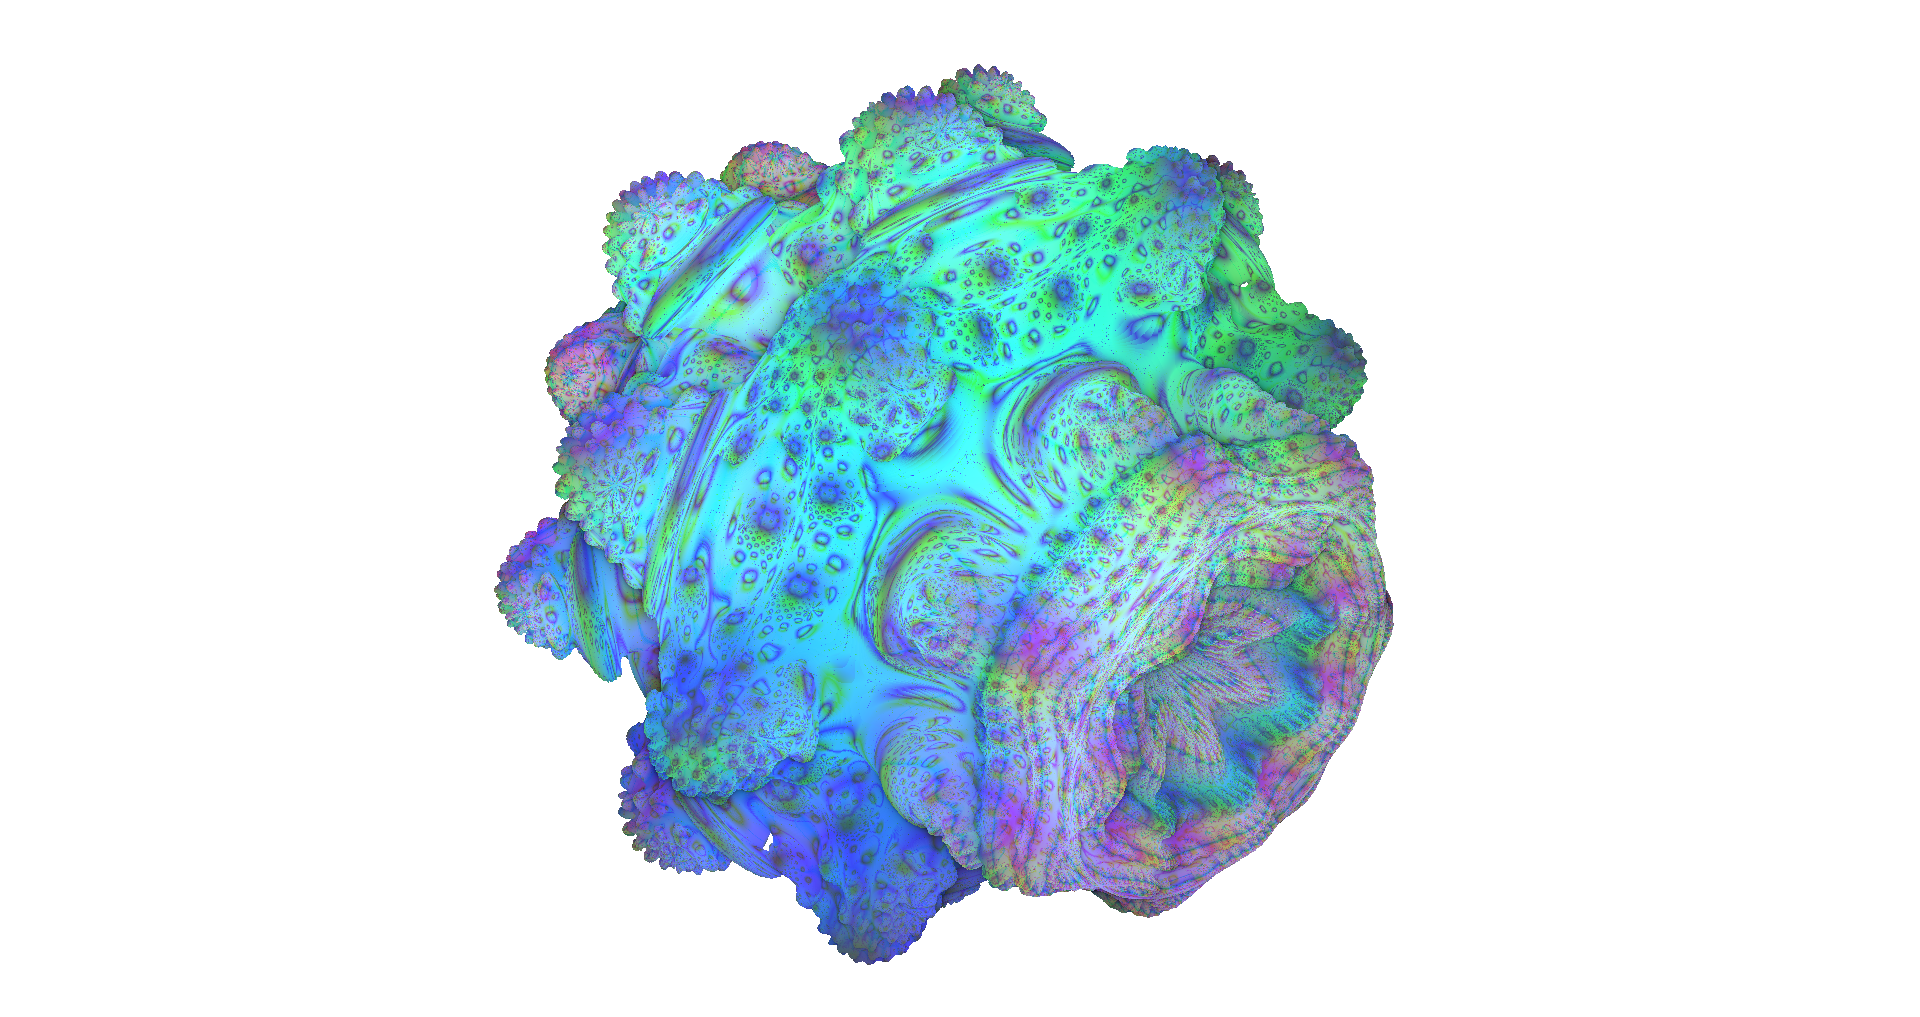
\includegraphics[width=\linewidth, frame]{Images/Results/Mandelbulb-View-01-Default.png}
		\caption{Mandelbulb: Default View.}
		\label{figure:mandelbulb-view-01-default}
	\end{subfigure}
	\hfill
	\begin{subfigure}[c]{0.45\linewidth}
		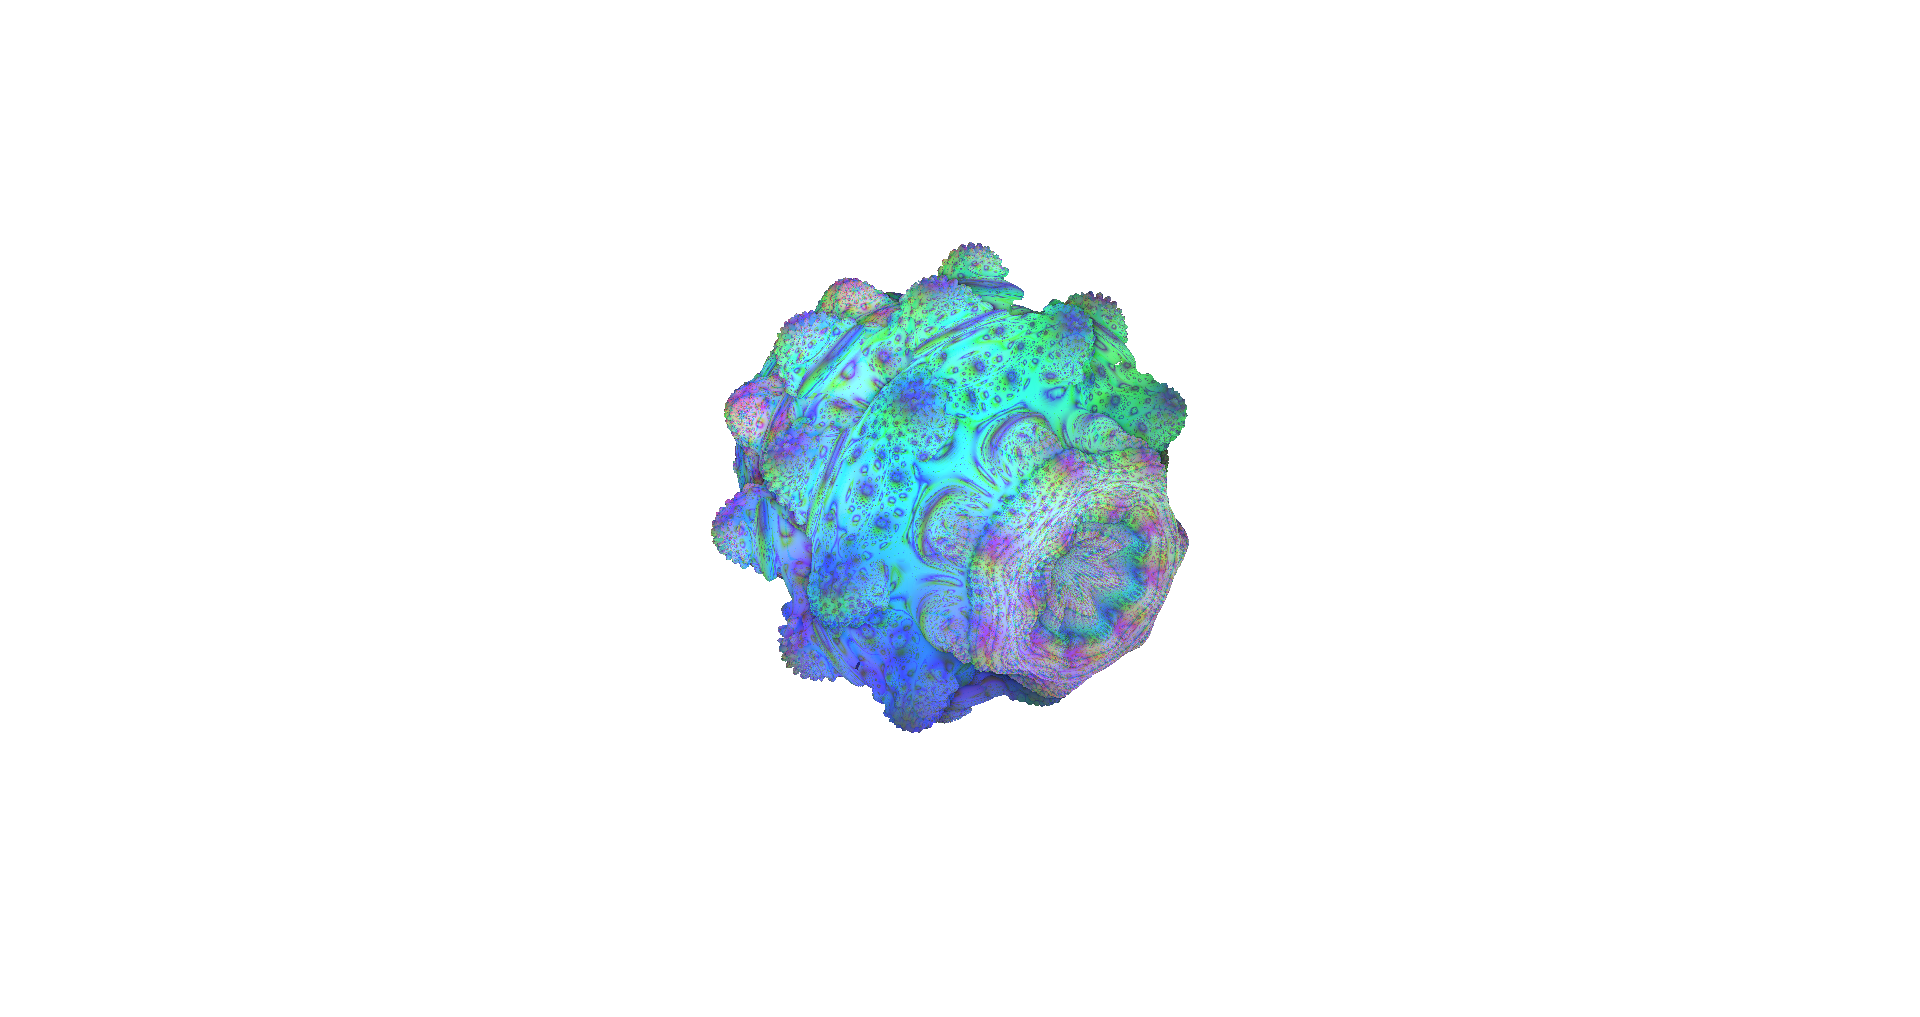
\includegraphics[width=\linewidth, frame]{Images/Results/Mandelbulb-View-02-Empty-Space.png}
		\caption{Mandelbulb: Zoomed Out View.}
		\label{figure:mandelbulb-view-02-empty-space}
	\end{subfigure}
	\hfill
	\begin{subfigure}[c]{0.45\linewidth}
		
\includegraphics[width=\linewidth, frame]{Images/Results/Mandelbulb-View-03-No-Space.png}
		\caption{Mandelbulb: Zoomed In View.}
		\label{figure:mandelbulb-view-03-no-space}
	\end{subfigure}
	\hfill
	\begin{subfigure}[c]{0.45\linewidth}
		
\includegraphics[width=\linewidth, frame]{Images/Results/Mandelbulb-View-04-Bottleneck.png}
		\caption{Mandelbulb: Bottleneck View.}
		\label{figure:mandelbulb-view-04-bottleneck}
	\end{subfigure}

	\caption{Four representative views of the Mandelbulb fractal, used in performance tests.}
	\label{figure:mandelbulb-views}
\end{figure}

Figure \ref{figure:mandelbulb-views} shows the four representative views used for performance measurements. Figure \ref{figure:mandelbulb-view-01-default} shows the default view, which is not expected to be particularly well suited to any performance measurement, to get a general-case overview of the performance differences between the methods used. Figure \ref{figure:mandelbulb-view-02-empty-space} is the view intended to include the most empty space (short of simply turning around and not looking at the fractal at all), and by contrast figure \ref{figure:mandelbulb-view-03-no-space} is intended to include the least. Lastly, figure \ref{figure:mandelbulb-view-04-bottleneck} includes a mix of depth and smoothness, and some bottlenecks.

\subsection{Expected Results}

The view of the Mandelbulb fractal involves quite a bit of empty space, unlike the Hall of Pillars fractal, which contains none. The expected result is that the Temporal caching method will give a slight performance boost to views with empty space, especially around the edges of the fractal, where more iterations would normally occur, but huge boosts are not expected since the Mandelbulb does not contain so many bottlenecks, and the depth variance is small. For still images, though, the temporal caching should give a boost no matter what is being looked at, as long as the camera does not move.\newline

For the signed distance field, it entirely depends on whether searching through the three-dimensional grid is less expensive than calculating the signed distance function or not, as the signed distance field is intended to provide a cheaper alternative every iteration, not to reduce the number of iterations as the temporal caching is supposed to do. The prediction is that the more costly the function, the more benefit will be seen, but that, since the Mandelbulb function is relatively cheap, there won't be much benefit, if any, with the distance function used here.

\subsection{Results}

\begin{table}[ht]
	\centering
	\begin{tabular}{||p{0.17\linewidth}|p{0.27\linewidth}|p{0.23\linewidth}|p{0.22\linewidth}||}
		\hline
		View & Unoptimized Time (ns) & SDF Difference (\%) & TC Difference (\%)\\
		\hline\hline
		Default & 1272832 & -154.38 & 2.06\\
		\hline
		Zoomed Out & 1083328 & -60.08 & 8.67\\
		\hline
		Zoomed In & 1241088 & -33.74 & -2.30\\
		\hline
		Bottleneck & 1593888 & -6.8 & 7.01\\
		\hline
	\end{tabular}
	\caption{A table showing the performance differences between the two optimization methods and the base, unoptimized rendering, for four different views of the Mandelbulb.}
	\label{table:mandelbulb-static-results}
\end{table}

Table \ref{table:mandelbulb-static-results} shows the results obtained for the four representative views of the Mandelbulb fractal. It shows the unoptimized time and the performance differences with the SDF and Temporal Caching (TC).\newline

Figure \ref{figure:mandelbulb-ao-results} shows the difference in the number of iterations using the unoptimized rendering and temporal cache methods, by colouring the fractal based on this number.

\begin{figure}[ht]
	\centering
	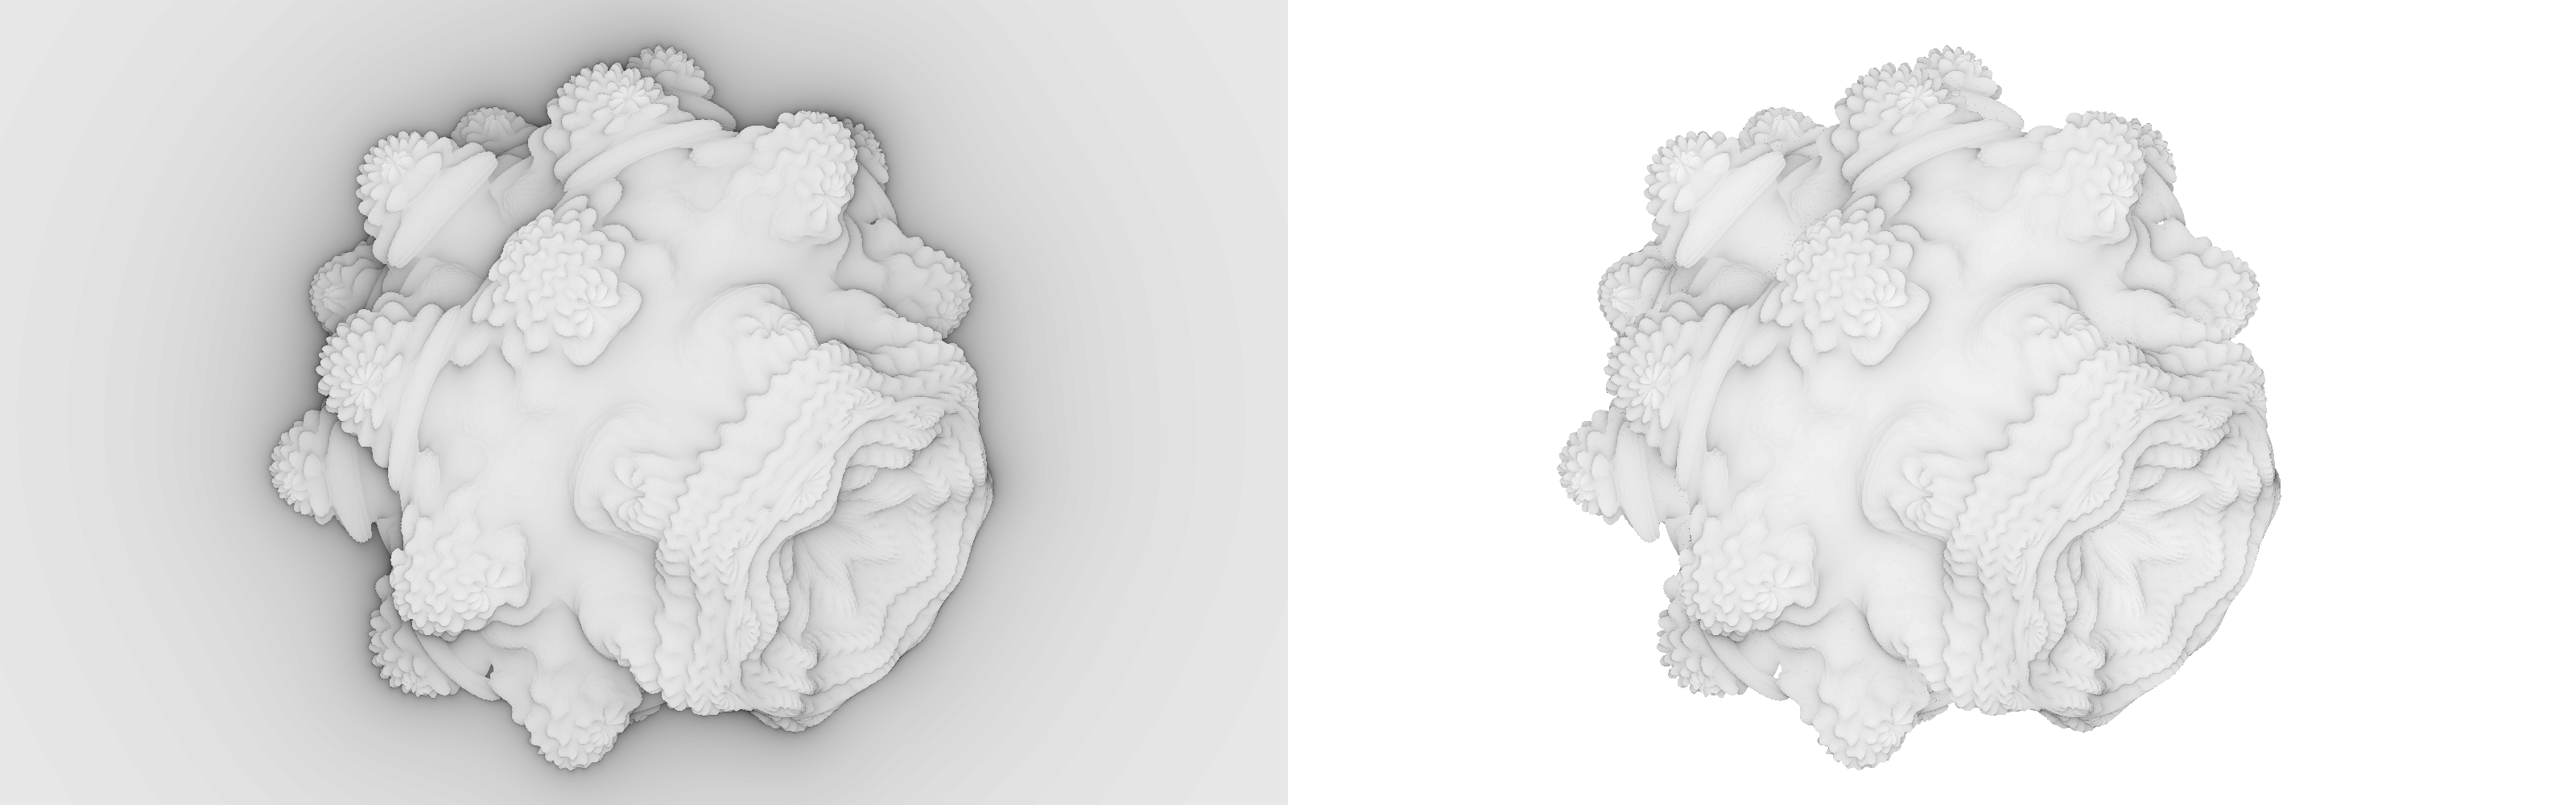
\includegraphics[width=\linewidth, frame]{Images/Results/Mandelbulb-AO-Results.png}
	\caption{The Mandelbulb, coloured based on the number of iterations achieved, rendered using the unoptimized method (left) and the temporal caching method (right).}
	\label{figure:mandelbulb-ao-results}
\end{figure}

\subsection{Evaluation}

Following the gathering of results, I decided to do a one-iteration performance measurement. In the shaders, I allowed one iteration of either the SDF search process, or the distance estimation, for the SDF shader and the unoptimized shader, respectively. The result was as expected; the render pass took 0.446ms with no optimizations, and 0.556ms with the SDF.

\subsubsection{Signed Distance Field}

Clearly, the signed distance field did not do well for this fractal, even though at first glance it seems a perfect fit for it, seeing as the whole fractal fits inside a reasonable boundary. I think overall, this is because the distance estimator for the Mandelbulb is so cheap, so the search through the SDF is outpaced by the distance function.\newline

The worst performance is seen with the default view. This may be because the whole fractal is visible, and fairly close to the camera, so fine detail is visible. This means that more iterations are needed, and most of them will fall within the cube, at least at first, making this the worst performer. Contrast that with the zoomed out view, where most of the rays fall outside the boundary of the SDF, which saves the performance a little, as the shader will revert to using the regular signed distance function if this happens. Additionally, less of the fractal is visible here, and in less detail. It seems that the performance measurements for the Mandelbulb simply show which of the views the SDF fights against the least.\newline

The zoomed in view is a little better. Considering the performance of the SDF so far, I think this view is better simply because it is closer to the fractal. This means that less iterations are done before the ray gets close enough to the surface of the fractal to begin using the regular signed distance function. I think the bottleneck view performed the best for a similar reason, with the addition that the surface is even simpler in this view, and the view out to the background is quite close to the edge of the SDF boundary, so it wouldn't be very many iterations once past the bottleneck to be free of the SDF cube.\newline

The SDF is not a suitable optimization for this fractal, in its current state. The process of searching through the SDF is clearly more expensive than the signed distance function calculation. If I were to use a more expensive fractal then maybe using the SDF would be worthwhile.

\subsubsection{Temporal Cache}

The temporal cache performed much better than the SDF, to the point where it actually gives a performance boost. The scenarios are also a little easier to explain. Starting with the zoomed in view, which decreased the performance. The surface in this view is quite detailed, and close to the camera. I think the performance difference was negative because of the deliberate underestimate that happens when using the saved distance. It is multiplied by 0.9, meaning that any iterations in that last 10\% are lost every frame. In this case, I think that most of the iterations happen in this last 10\%, where the surface becomes more complex, so the temporal cache provides no benefit here. The negative difference most likely comes from the overhead involved in sampling from the texture image, and the extra comparisons that happen for the camera movement test, for example.\newline

The largest performance difference came from the zoomed out view. I was expecting it to come from the bottleneck, but I suppose that in terms of edges, the zoomed out view contains just as many. In addition, the empty space will also receive a boost, and not just around the edges, so a large part of the performance increase likely comes from here. As well as this, less of the fractal surface is visible, so although the problem present in the zoomed in view applies, and most of the iterations for the surface come from that last 10\% that is cut out, the portion of the image to which this applies is very small in this view.\newline

The performance for the default view lines up with the explanations for the zoomed out and zoomed in views. There is more empty space, and there are more edges, in the default view than in the zoomed in view, so the performance will be better, but there is also more surface space, which this optimization method does not perform well on, so that will cause a hit to overall performance.\newline

This drawback does not apply so much to the bottleneck scenario, despite it being close to the surface. There is not a lot of complicated geometry in this view, so the cut to iteration progress doesn't hit the performance so hard. Most of the performance boost probably comes from the avoidance of the obvious bottleneck (hole) in the middle, and the smaller one on the right.\newline

Figure \ref{figure:mandelbulb-ao-results} shows a distinct reduction in the number of iterations using the temporal caching method, especially in the background and at the edges of the Mandelbulb. However, during testing the image did flicker, especially in the background. I think this is because of the view distance limit. The rays will travel a little further each frame, which triggers the ray recasting. If this was fixed, then one might expect better performance from the temporal cache. Overall, the temporal cache is worth using for the Mandelbulb fractal, even though there are some improvements to be made.

\section{Mandelbulb Animation Test}

This section will examine the performance while animating the Mandelbulb by changing its parameter. Recall figure \ref{figure:mandelbulb-powers} in chapter \ref{chapter:implementation}. It shows the Mandelbulb, raised to different powers. This power is the parameter that is varied in the animation.

\subsection{Animation}

The animation of the Mandelbulb parameter takes a total of 8000 frames. The parameter starts at 10 and gets raised to 16 by the end of the first 2000 frames. Then, it decreases to 4 over 4000 frames. Finally, over 2000 frames it returns to 10. Refer back to figure \ref{figure:mandelbulb-powers} in chapter \ref{chapter:implementation} for an overview of how this looks.

\subsection{Expected Results}

I don't have solid predictions for this animation. I expect to see some gains in some sections, and perhaps some losses in others. Any section of the animation that is visually slower will perhaps trigger the ray recast mechanism less, so there would be gains here. Any faster animation, and the performance may stay the same or decrease. Any part of the animation that involves more empty space will likely see gains, based on the results for the static images.

\subsection{Results}

\begin{figure}[ht]
	\centering
	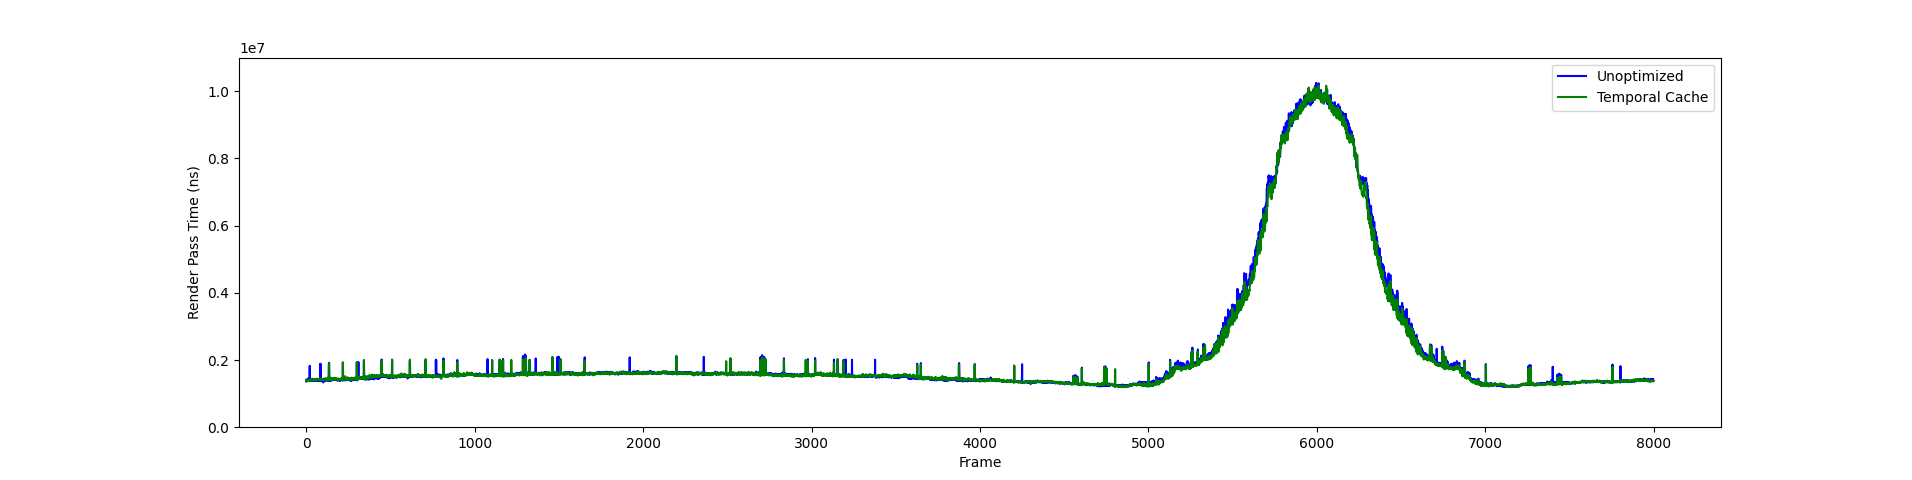
\includegraphics[width=\linewidth, frame]{Images/Results/Mandelbulb-Parameter-Animation.png}
	\caption{A graph showing the render pass time during an animation of the Mandelbulb parameter, for both unoptimized rendering and rendering using the temporal cache.}
	\label{figure:mandelbulb-parameter-animation}
\end{figure}

Figure \ref{figure:mandelbulb-parameter-animation} shows the graph of the render pass time over the animation. It is very difficult to see if there are performance differences anywhere in the animation from this, as the two lines overlap almost exactly, but it's useful to know where the performance changes overall during the animation. Figure \ref{figure:mandelbulb-parameter-animation-gain} shows a plot of the performance difference over the animation, with a line of best fit plotted to make it clearer (the line of best fit ignores the large spikes in the data).

\begin{figure}[ht]
	\centering
	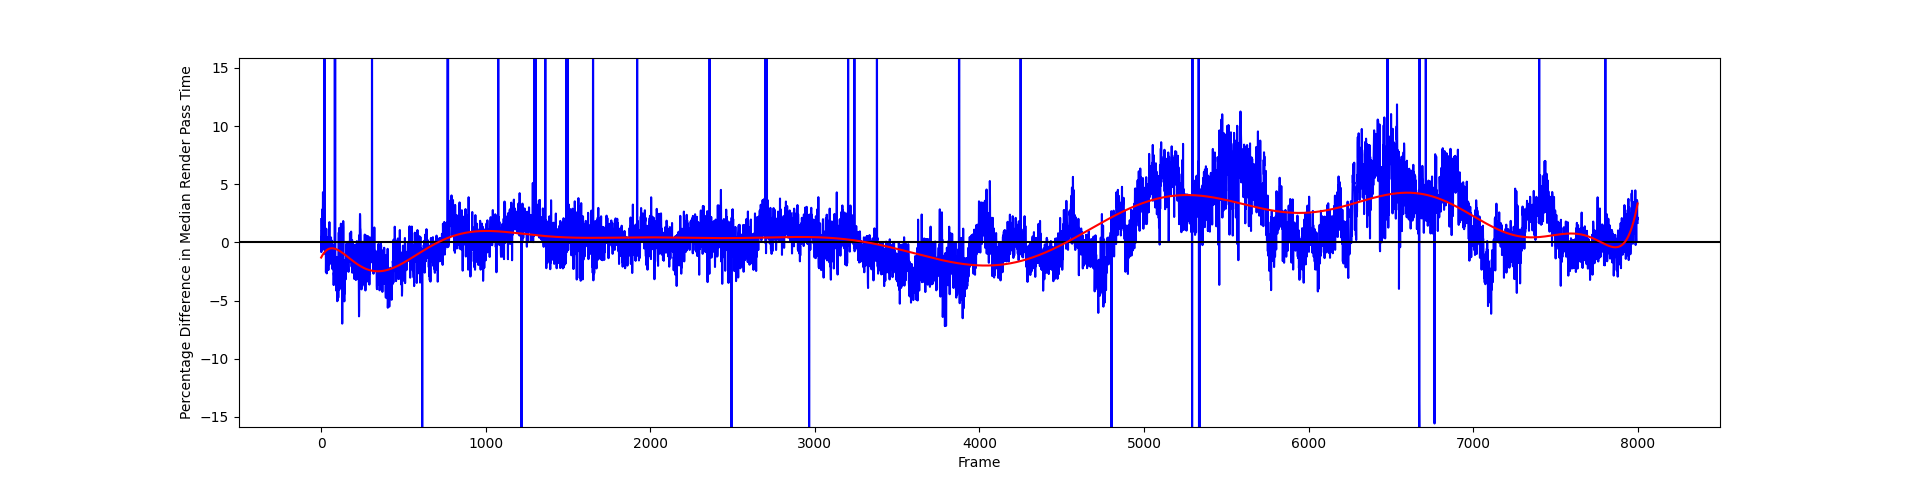
\includegraphics[width=\linewidth, frame]{Images/Results/Mandelbulb-Parameter-Animation-Gain.png}
	\caption{A graph showing the performance difference during an animation of the Mandelbulb parameter, between unoptimized rendering and rendering using the temporal cache. Positive values mean that the temporal cache performs better.}
	\label{figure:mandelbulb-parameter-animation-gain}
\end{figure}

\subsection{Evaluation}

The main surge in render pass time, in figure \ref{figure:mandelbulb-parameter-animation}, comes about when the parameter is approaching its lowest value. The number of iterations required to reach the surface increases because the surface becomes more intricate. This difference can actually be seen in the image from chapter \ref{chapter:implementation}, figure \ref{figure:mandelbulb-powers}. The image on the left is noticeably darker. This is because the image colouring is done in combination with the ambient occlusion effect described. There is a greater portion of smooth surface, as well as empty space, at this point.\newline

Around the same time as the surge in render pass time, there is a general increase in the performance benefit received from the temporal cache. I believe this is because of the extra smooth surface and empty space, as described. The animation is moving at the same speed, but the changes in the landscape are less from frame to frame. Contrast this with the times around frames 0/8000 and 4000. This is where the parameter reaches 10, which is the starting value. At this point, the landscape is changing the quickest, with new geometry occluding the old at high rates, and less empty space. When the parameter reaches its peak, 16, at frame 2000, these occlusions are still happening, but at a lower rate, so the performance does not dip in the same way as when the animation is at its fastest in terms of occlusion.\newline

Overall the temporal cache performs quite well during the animation, despite, at times, rapid changes in geometry. Additionally, there are more gains than losses, and the losses are smaller than the gains.

\section{Hall of Pillars Static Image Tests}

\subsection{Representative Views}

\begin{figure}[ht]
	\centering

	\begin{subfigure}[c]{0.3\linewidth}
		
\includegraphics[width=\linewidth, frame]{Images/Results/Hall-Of-Pillars-View-01-Default.png}
		\caption{Hall of Pillars: Default View.}
		\label{figure:hall-of-pillars-view-01-default}
	\end{subfigure}
	\hfill
	\begin{subfigure}[c]{0.3\linewidth}
		\includegraphics[width=\linewidth, frame]{Images/Results/Hall-Of-Pillars-View-02-Large-Hall.png}
		\caption{Hall of Pillars: Large Hall View.}
		\label{figure:hall-of-pillars-view-02-large-hall}
	\end{subfigure}
	\hfill
	\begin{subfigure}[c]{0.3\linewidth}
		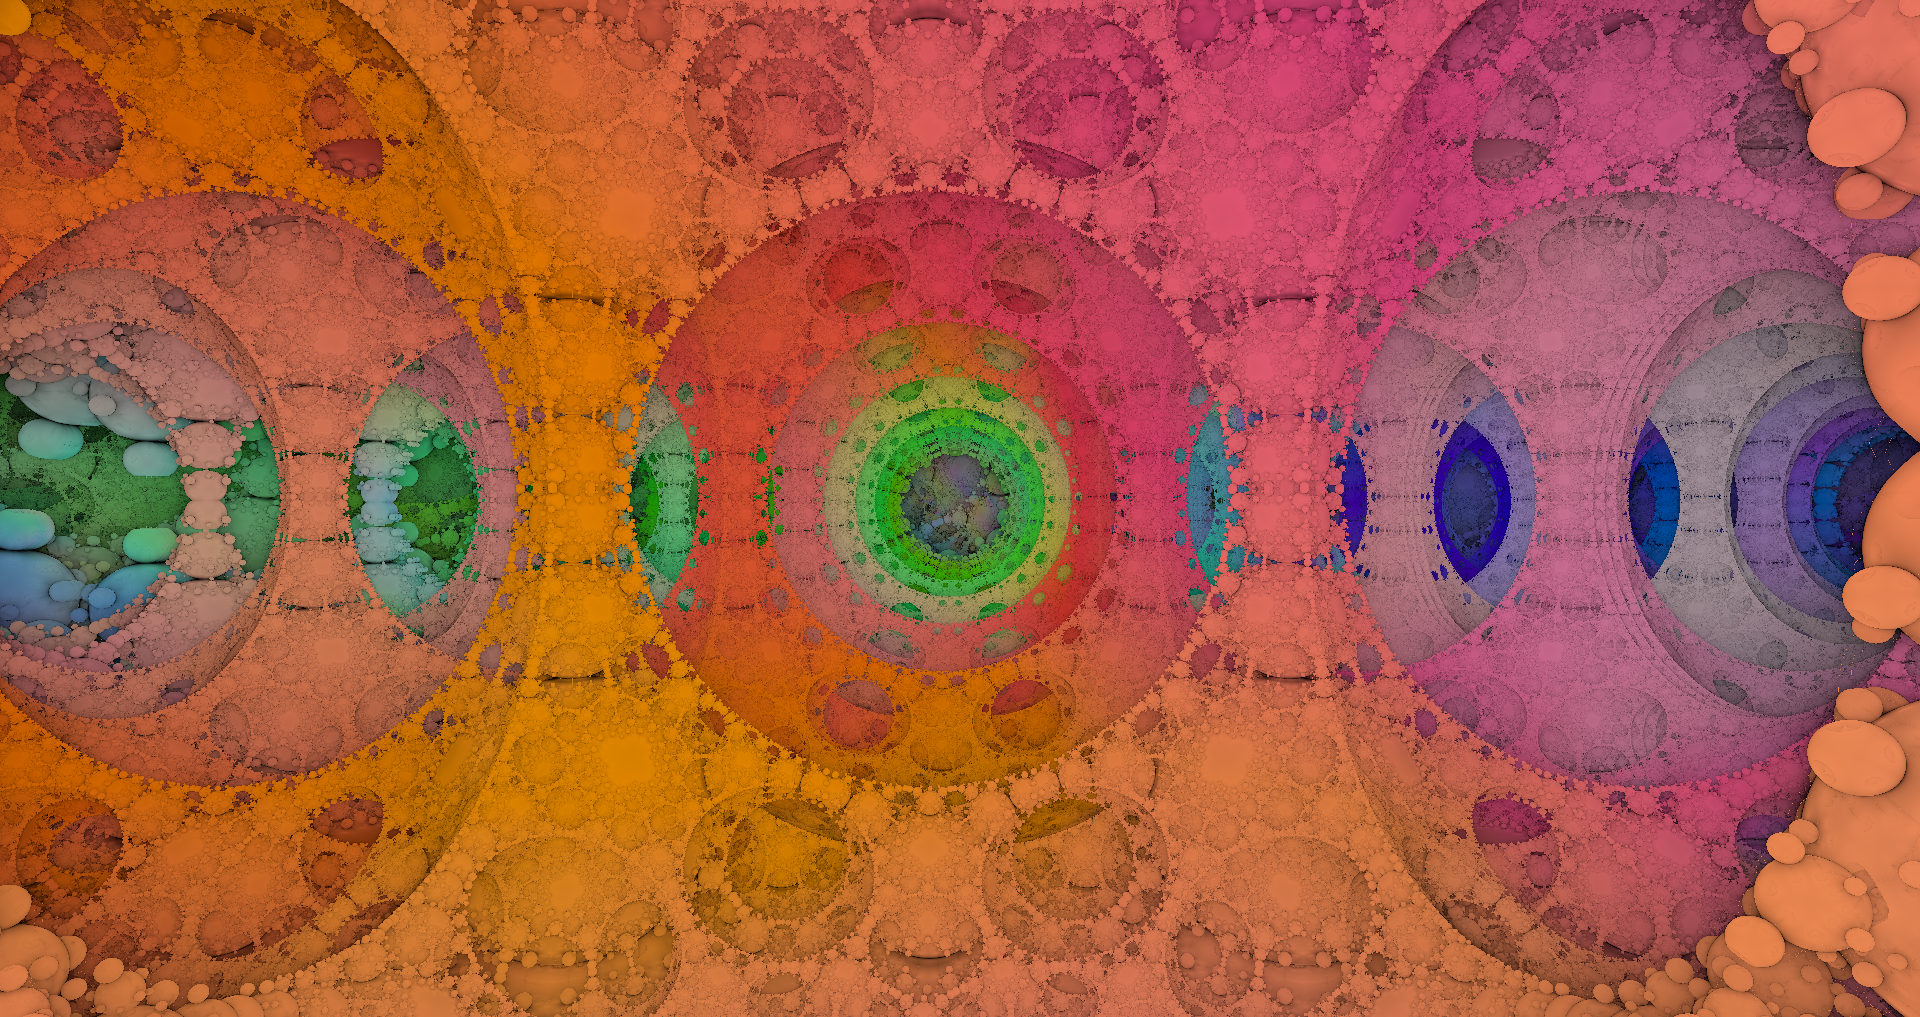
\includegraphics[width=\linewidth, frame]{Images/Results/Hall-Of-Pillars-View-03-Corridor-Of-Bottlenecks.png}
		\caption{Hall of Pillars: Bottleneck Corridor View.}
		\label{figure:hall-of-pillars-view-03-bottleneck-corridor}
	\end{subfigure}
	\hfill
	\begin{subfigure}[c]{0.3\linewidth}
		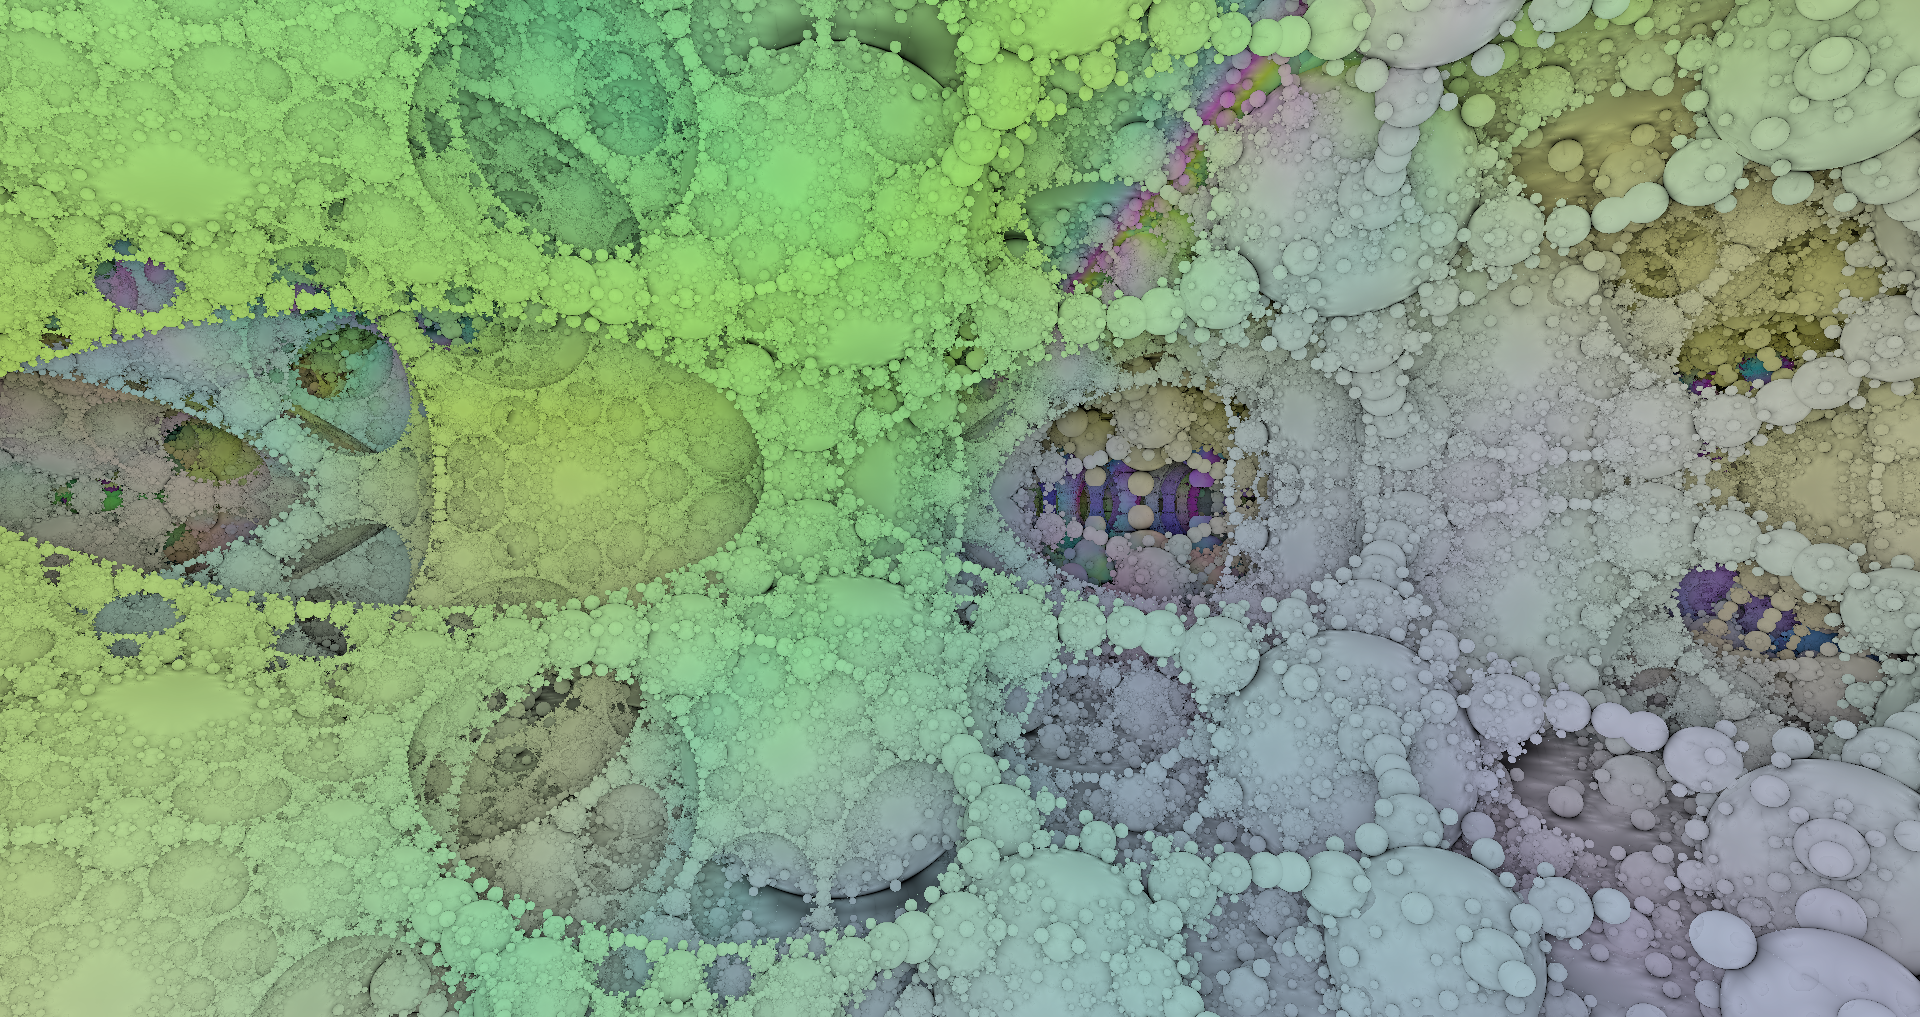
\includegraphics[width=\linewidth, frame]{Images/Results/Hall-Of-Pillars-View-04-Intricate-Geometry.png}
		\caption{Hall of Pillars: Intricate Geometry View.}
		\label{figure:hall-of-pillars-view-04-intricate-geometry}
	\end{subfigure}
	\hfill
	\begin{subfigure}[c]{0.3\linewidth}
		
\includegraphics[width=\linewidth, frame]{Images/Results/Hall-Of-Pillars-View-05-Simple-Geometry.png}
		\caption{Hall of Pillars: Simple Geometry View.}
		\label{figure:hall-of-pillars-view-05-simple-geometry}
	\end{subfigure}

	\caption{Five representative views of the Hall of Pillars fractal, used in performance tests.}
	\label{figure:hall-of-pillars-views}
\end{figure}

Figure \ref{figure:hall-of-pillars-views} shows the representative views chosen for the Hall of Pillars fractal. These were chosen to vary greatly in depth and complexity. Given the theory on why the temporal cache should give a performance boost (bottlenecks), images \ref{figure:hall-of-pillars-view-01-default} and \ref{figure:hall-of-pillars-view-02-large-hall} were chosen to provide an average case, images \ref{figure:hall-of-pillars-view-03-bottleneck-corridor} and \ref{figure:hall-of-pillars-view-04-intricate-geometry} were chosen as best cases, and finally \ref{figure:hall-of-pillars-view-05-simple-geometry} was chosen as a worst case. These views also provide good variety for testing the SDF. All but the `Large Hall' view are mostly encompassed by the SDF; the Hall is just too large in scale to be covered adequately.

\subsection{Expected Results}

This fractal contains many bottlenecks (the ray has to pass close to lots of geometry before reaching any surface), so the temporal caching method is expected to perform better here than with the Mandelbulb, in terms of performance difference. A view with very simple geometry was also chosen because of this, as the prediction is that the temporal caching method will provide minimal benefit where these bottlenecks don't exist or the surface is very smooth.\newline

The signed distance field is being used in a somewhat different scenario compared to the Mandelbulb. This fractal doesn't seem to be finite, so only a relatively small area can be covered by the SDF, which makes testing tricky. A ray culling step was tried, to stop any ray which ventures outside the main SDF cube (including in shaders that aren't using the 3D SDF, for consistency) but this did not yield significantly different results to using it as normal, and just allowing the rays to travel outside the box. It was also not representative of the kind of uses for this fractal. Especially in the `Large Hall' view, in which the SDF can only cover a segment of one pillar. I predict that, like with the Mandelbulb, this will not perform well, as the Hall of Pillars distance estimator is not significantly more expensive than the Mandelbulb one.

\subsection{Results}

\begin{table}[ht]
	\centering
	\begin{tabular}{||p{0.24\linewidth}|p{0.27\linewidth}|p{0.22\linewidth}|p{0.22\linewidth}||}
		\hline
		View & Unoptimized Time (ns) & SDF Difference (\%) & TC Difference (\%)\\
		\hline\hline
		Default & 7524352 & -2.08 & 24.02\\
		\hline
		Large Hall & 12879840 & -1.39 & 12.43\\
		\hline
		Bottleneck Corridor & 10053440 & -10.76 & 26.07\\
		\hline
		Intricate Geometry & 10091680 & -8.04 & 25.62\\
		\hline
		Simple Geometry & 1176352 & -4.76 & 12.39\\
		\hline
	\end{tabular}
	\caption{A table showing the performance differences between the two optimization methods and the base, unoptimized rendering, for five different views of the Hall of Pillars fractal.}
	\label{table:hall-of-pillars-static-results}
\end{table}

As before, table \ref{table:hall-of-pillars-static-results} shows the raw time for the render pass in the unoptimized rendering, as well as performance differences for the SDF and temporal caching (TC) methods, and figure \ref{figure:hall-of-pillars-ao-results} shows the differences in the number of iterations achieved.

\begin{figure}[ht]
	\centering
	\includegraphics[width=\linewidth, frame]{Images/Results/Hall-Of-Pillars-AO-Results.png}
	\caption{The Hall of Pillars fractal, coloured based on the number of iterations achieved. Each image is split in two; the left half is rendered using the unoptimized method, and the right half uses the temporal cache. The lighter the image, the better the performance.}
	\label{figure:hall-of-pillars-ao-results}
\end{figure}

\subsection{Evaluation}

\subsubsection{Signed Distance Field}

Compared to the SDF performance for the Mandelbulb, the SDF here performed extremely well, though it still reduced performance in all cases. I think that if the Hall of Pillars distance estimator was more expensive to evaluate, there may have been some positive results. That being said, the SDF was comparatively a lot more coarse than for the Mandelbulb, though it did benefit from an extra subdivision level. I did try changing the subdivision level from 9 to 8, but this did not result in a performance difference.\newline

I think that perhaps for scenes that cross a great deal of the SDF, the shaders are likely to encounter a lot more cache misses, as the total size of the SDF in these tests was 512MB. This will lower performance for scenes such as this. If the subdivision level is too low, and the SDF stretched across too much space, then the voxels will be large, and it will be easier to get past the SDF search stage to fall back on the regular signed distance function. Recall figure \ref{figure:sdf-hybrid-comparison} from chapter \ref{chapter:implementation}. The SDF is clearly a lot more coarse for the Hall of Pillars, in order to cover any kind of decent distance. Another level of subdivision was not possible due to memory constraints. I think this is one reason for the `increase' in performance compared to the Mandelbulb; it simply did not get in the way as much. This is evidenced by the fact that in the view in which it covers the least ground, the Large Hall, we have the smallest performance loss.\newline

Further evidence for this claim is the result for the Bottleneck Corridor view. This view contains a great deal of tunnels and holes in the scene. This view was chosen because I thought it might slow the rays down the most, and therefore result in the greatest performance gain for the temporal cache. It has also resulted in the greatest performance loss for the SDF. The scale of this view means that most of it is contained inside the SDF. This is the worst case out of the views. Lots of bottlenecks, almost all of which are inside the SDF. The Intricate Geometry view has a very similar problem; almost all of that is contained inside the SDF as well (this goes for all views except the Large Hall).\newline

Overall, although the SDF performed better than with the Mandelbulb, I believe this to be an illusion. It is not suitable for use in its current state.

\subsubsection{Temporal Cache}

In contrast to the SDF, the results for the temporal cache were much improved over those it achieved on the Mandelbulb. Even the worst case view resulted in a 12.39\% performance gain. However, this is for a static image, and much of the gain is likely to be lost during movement (more on that in the next section). There isn't much to explain with these results. They are as expected, and likely for the reasons predicted; the presence of a large number of bottlenecks in the scene, and complex geometry. The worst performers were the view with the simplest geometry, as expected, but also the one with the largest view distance (`Large Hall'). This was surprising, as the scene does contain a lot of bottlenecks.\newline

Figure \ref{figure:hall-of-pillars-ao-results} shows the comparison between the number of iterations achieved with unoptimized rendering and the temporal cache, for each of the representative views. The differences seem to match up with the data obtained. The difference is particularly stark for the Bottleneck Corridor view and the Intricate Geometry view. During rendering, the same flickering happened in the background of the Large Hall view as it did for the Mandelbulb, which may be why, despite there being a lot of bottlenecks in the scene, the performance wasn't better. I did expect this view to yield more of a benefit than it did.\newline

The temporal caching method is particularly well suited to this fractal. The next section will explore how much of the performance gain can be preserved with movement.

\section{Hall of Pillars Animation Tests}

\subsection{Animations}

Two animations were constructed for the Hall of Pillars fractal. One is a flythrough of several scenes, and the other is an animation resulting from varying a parameter in the distance function. Refer back to figure \ref{figure:glsl-distance-estimator-hall-of-pillars} in chapter \ref{chapter:implementation} to see the use of the fractal parameter in the distance estimation.

\subsubsection{Flythrough}

\begin{figure}[ht]
	\centering
	\includegraphics[width=\linewidth, frame]{Images/Results/Hall-Of-Pillars-Flythrough-Guide.png}
	\caption{Key frames in the Hall of Pillars flythrough animation. They are in order, left to right, top to bottom. The frames at which they occur are written on each image.}
	\label{figure:hall-of-pillars-flythrough-guide}
\end{figure}

Figure \ref{figure:hall-of-pillars-flythrough-guide} provides a guide to the progress of the animation at key points. To give a sense of scale, any image in which you can see white is a scene where the view distance limit (which is just over sixteen thousand) is exceeded. The first four images have a range of approximately five hundred. The penultimate image is of the top of a pillar; a corresponding structure can be seen at the top of the image preceding it (frame 10,000). The last image is inside the top of this structure. The images shown are key images in relation to the graph of performance that will be shown in the results section. These will be explained there, but refer back to this image to aid in understanding what is happening during the animation to cause fluctuations in performance, and performance gain.

\subsubsection{Parameter Animation}

\begin{figure}[ht]
	\centering
	\includegraphics[width=\linewidth, frame]{Images/Results/Hall-Of-Pillars-Parameter-Guide.png}
	\caption{Key stages in the Hall of Pillars parameter animation. The parameter values are as follows, left to right, top to bottom: 1.6, 1.8, 2.0, 2.2 and 2.4.}
	\label{figure:hall-of-pillars-parameter-guide}
\end{figure}

Figure \ref{figure:hall-of-pillars-parameter-guide} shows a guide for the stages of the parameter animation. The sequence starts in the middle (the third image) and moves towards the scene in the last image. Then, the animation reverses and morphs in to the first image. Finally, it moves back to the start. The first image is so dark because the scene takes progressively more iterations to render as the parameter decreases, and these images are rendered with the `ambient occlusion' effect previously mentioned.

\subsection{Expected Results}

I expect to see a performance gain over some of the flythrough animation - particularly sequences in which movement is slow, and there is no camera movement. I don't expect to see a gain where there is movement, combined with complex geometry, or a lot of camera movement; recipes for lots of occlusion and ray recasting.\newline

For the parameter animation, the view is much more stable, given that the camera doesn't move at all, but the geometry changes. With this in mind, I expect performance somewhere between the static images and the flythrough animation.

\subsection{Results - Flythrough}

\begin{figure}[ht]
	\centering
	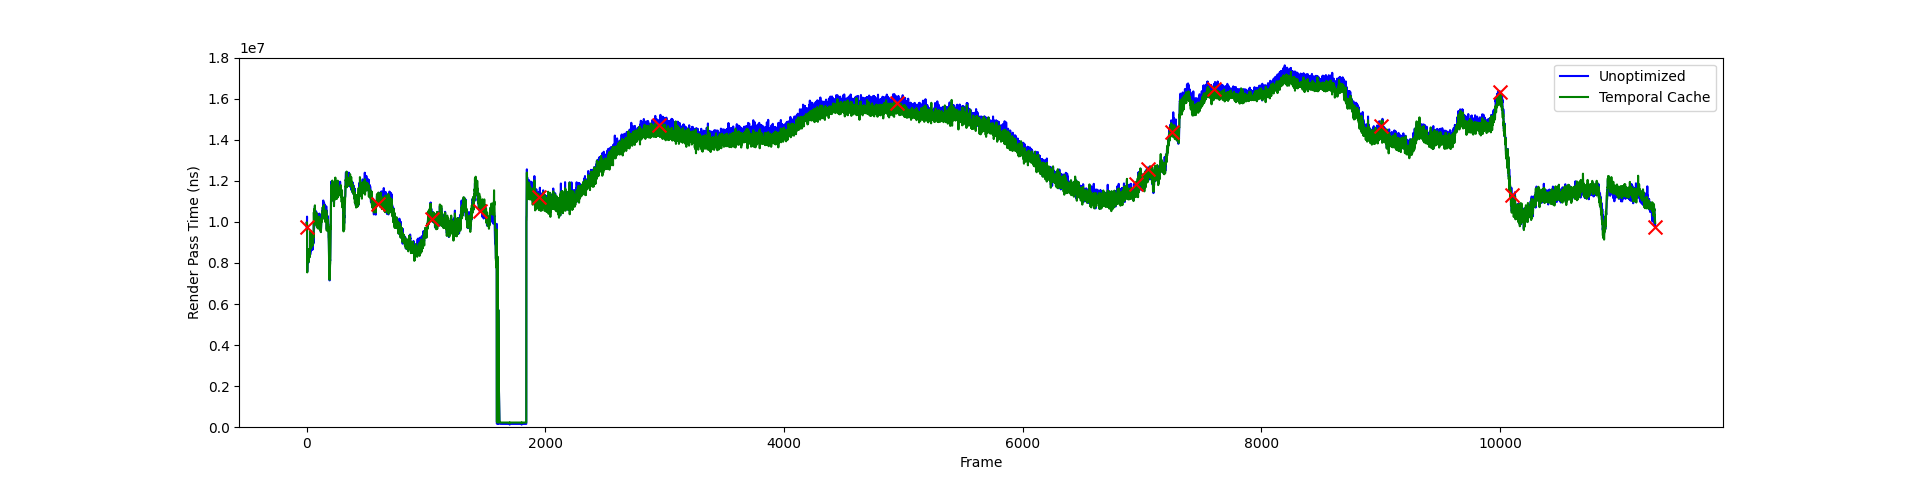
\includegraphics[width=\linewidth, frame]{Images/Results/Hall-Of-Pillars-Flythrough-Animation.png}
	\caption{A graph showing the render pass time during a flythrough animation of the Hall of Pillars, for both unoptimized rendering and rendering using the temporal cache. The red X marks indicate key frames for the animation.}
	\label{figure:hall-of-pillars-flythrough-animation}
\end{figure}

\begin{figure}[ht]
	\centering
	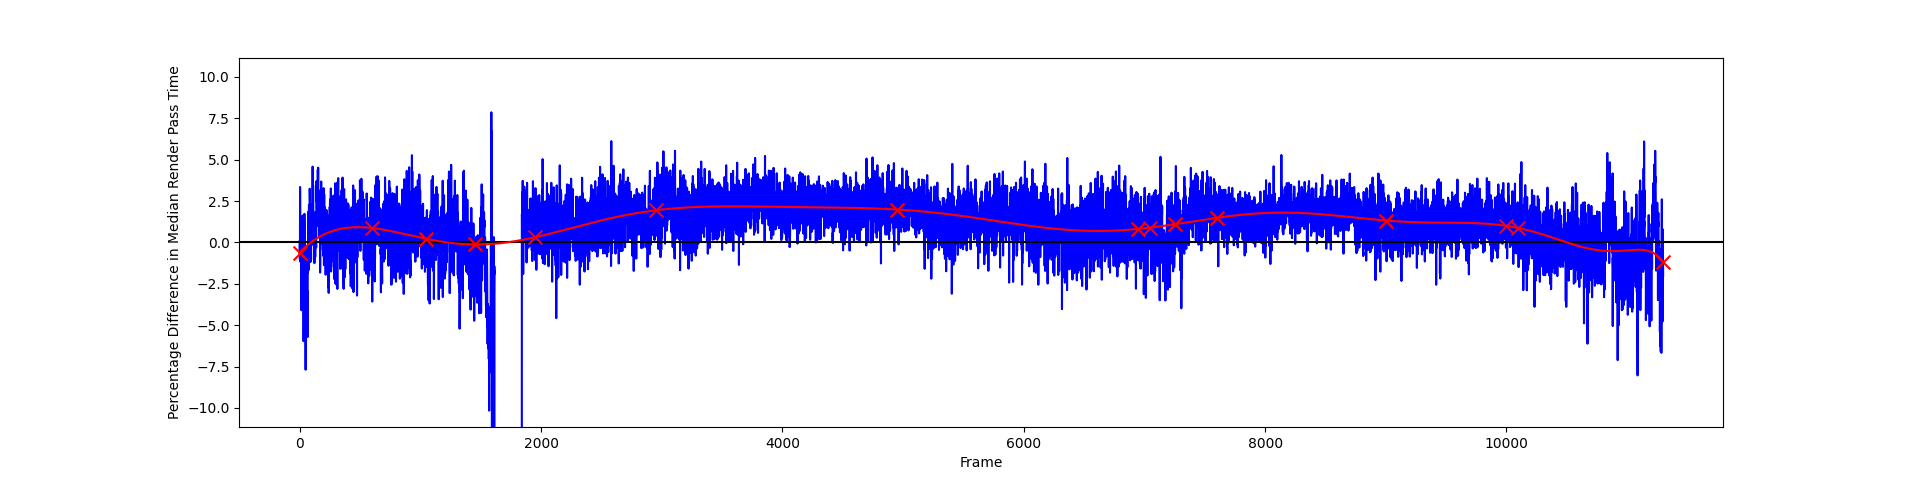
\includegraphics[width=\linewidth, frame]{Images/Results/Hall-Of-Pillars-Flythrough-Animation-Gain.png}
	\caption{A graph showing the performance difference during a flythrough animation of the Hall of Pillars, between unoptimized rendering and rendering using the temporal cache. Positive values mean that the temporal cache performs better. The red X marks indicate key frames for the animation.}
	\label{figure:hall-of-pillars-flythrough-animation-gain}
\end{figure}

Figure \ref{figure:hall-of-pillars-flythrough-animation} shows the graph of the render pass time over the animation. A small performance difference can be seen here (where the blue line is visible above the green one), despite the general noisiness due to the changing landscape. The sharp drop in time just before frame 2000 corresponds with the camera moving through the `ceiling' of one of the rooms in the fractal. During this time, the number of iterations will drop to 1 or close to 1, as the camera is inside the shape. The time drops close to zero, but this was not considered an interesting part of the animation, so it is cut off a bit in these graphs. Perhaps it is interesting to note, however, the drop in performance around that time (see figure \ref{figure:hall-of-pillars-flythrough-animation-gain}). This is likely because of the overhead involved in sampling the texture image, and the extra calculations, for no reduction in iteration count.

Figure \ref{figure:hall-of-pillars-flythrough-animation-gain} confirms the observation of a performance boost. A positive difference in performance can be observed over most of the animation, meaning that even for scenes with more rapid movement, the temporal cache still maintains its advantage.

\subsection{Evaluation - Flythrough}

Surprisingly, the temporal cache managed to provide a performance benefit throughout the animation, though it was much reduced. It seems to fluctuate mostly between approximately 1\% and 2.5\%. This is a huge reduction from the numbers seen for the static images, but was to be expected.\newline

The sequence between frames 0 and 600 involves fairly quick movement, but slow camera rotation. There is also a lot of complex geometry in this sequence, mixed with some flat surfaces. I think the performance increases during this sequence because the flat areas can be seen through bottlenecks. The combination of these things means that there is a bottleneck-related performance gain, and the frame-to-frame distance doesn't change too much.\newline

After this sequence, the camera dive into one of the holes near the ground. The geometry becomes less complicated during this time, and the distance from the camera to any surface decreases. Not much performance benefit can be seen here as a result. After this, as mentioned, the camera goes through the ceiling, which results in a dramatic decrease in performance. Upon emerging on the other side, the image in frame 1950 (top-right in figure \ref{figure:hall-of-pillars-flythrough-guide}) can be seen. The camera is still moving, and a large portion of the bottlenecks in this particular scene are near the end of the ray's journey, so some of the performance benefit will be lost due to the deliberate underestimate.\newline

The camera then pans across the ceiling of this large hall to end up at the view in frame 2950. During this sequence the performance increases to its highest level. The camera movement is very slow, as is the rotation, and the movement brings into focus a scene more suited to the strengths of the temporal cache. This scene slowly evolves for 2000 frames until the view in frame 4950. The performance benefit is maintained for this entire duration. This sequence has the best performance for the temporal cache. I think this is due to the very slow movement and rotation, and the temporal cache-friendly scenery.\newline

The performance dips after this, as the camera takes another dive into the base of the right-hand pillar. The geometry contains less bottlenecks and complexity for this sequence, but the camera rotation and movement is still slow, so performance stays in the positive. Here, there is a sequence where the camera moves quickly through a couple of `tunnels', to emerge in another area with a large amount of complex geometry and high view distance, resulting in the second best performance at around frame 7600.\newline

After this, the movement is quite slow, but there are a couple of fast, 90 degree turns of the camera between frames 7600 and 10000. Still, the temporal cache manages to maintain overall positive performance. The performance really suffers when zooming in to the top of a pillar near the end of the sequence. As you can see from the last image, the geometry is simple, and since the camera is moving and rotating at a moderate rate, the ray casting mechanism will be triggered quite often.\newline

Overall the temporal cache holds up well with movement and doesn't completely deteriorate, but much more work is needed to boost the performance during movement. I think a better, more reliable way to detect occlusion would allow for a closer estimate of the true distance, reduce the need for such a harsh underestimate during sampling, and help to trigger ray recasting a lot less often.

\subsection{Results - Parameter Animation}

\begin{figure}[ht]
	\centering
	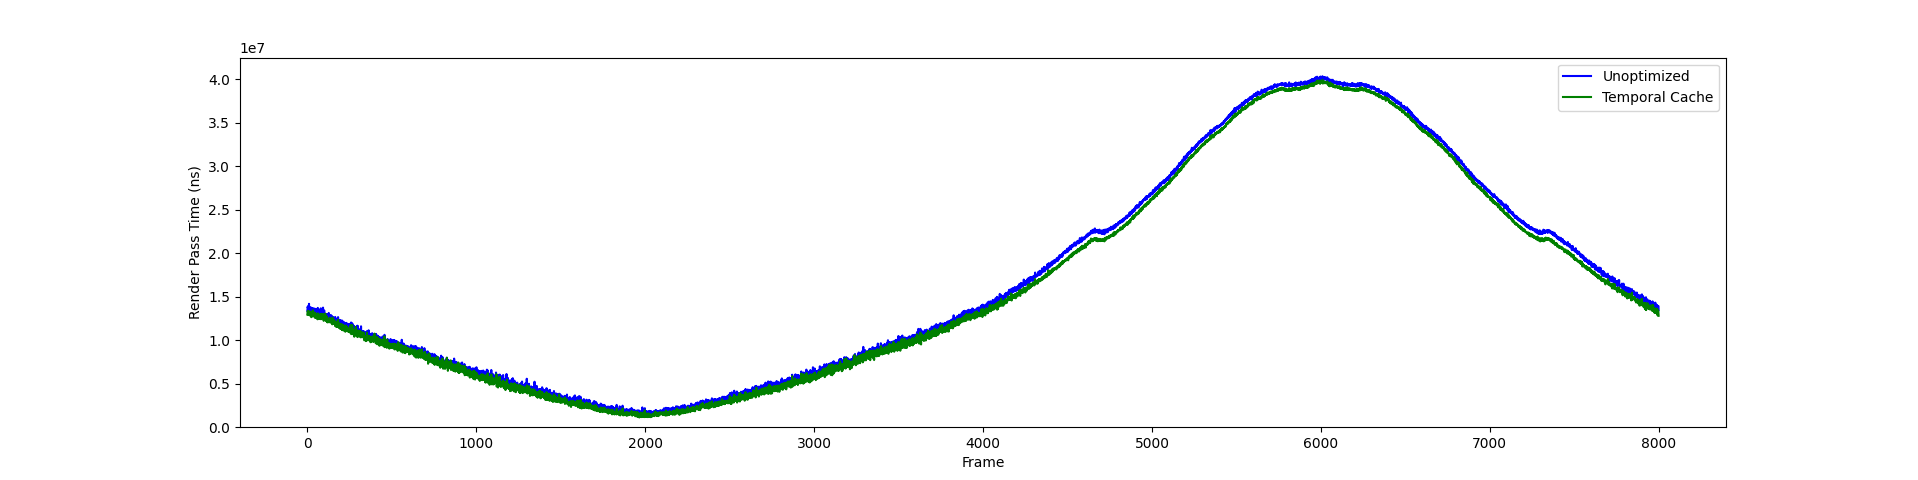
\includegraphics[width=\linewidth, frame]{Images/Results/Hall-Of-Pillars-Parameter-Animation.png}
	\caption{A graph showing the render pass time during an animation of the Hall of Pillars parameter, for both unoptimized rendering and rendering using the temporal cache.}
	\label{figure:hall-of-pillars-parameter-animation}
\end{figure}

\begin{figure}[ht]
	\centering
	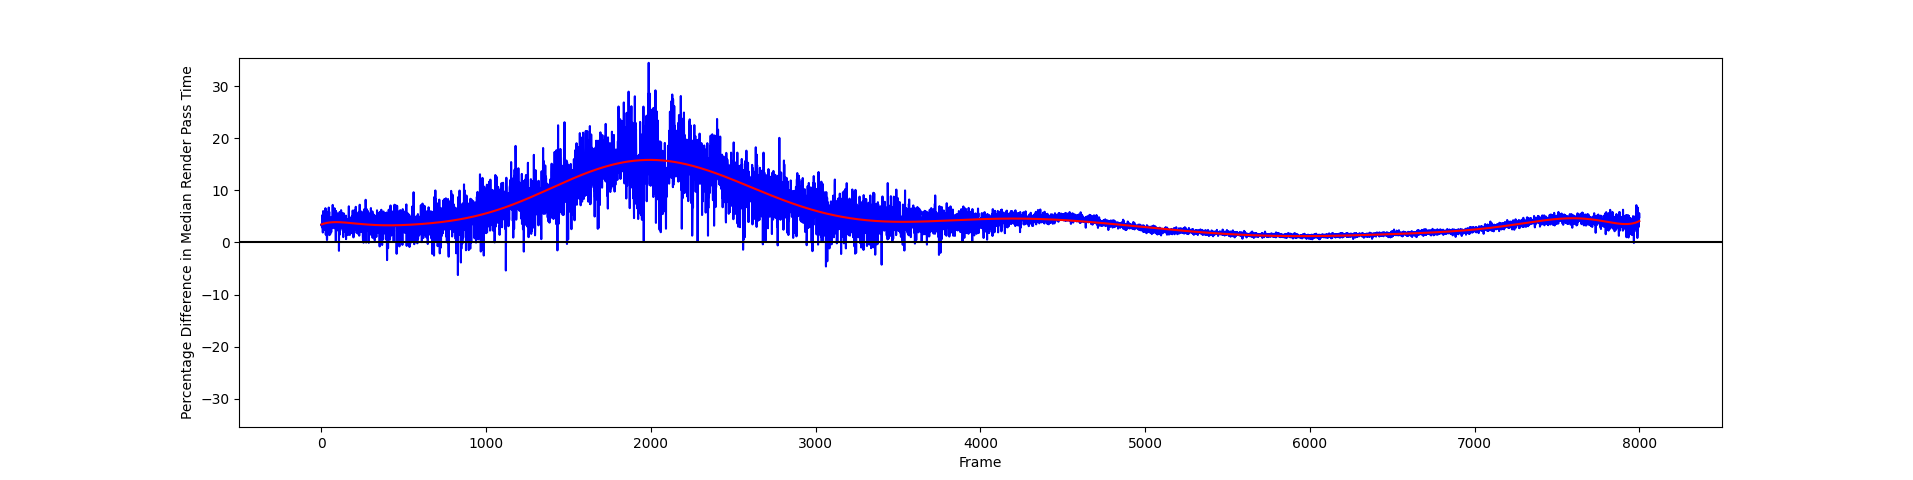
\includegraphics[width=\linewidth, frame]{Images/Results/Hall-Of-Pillars-Parameter-Animation-Gain.png}
	\caption{A graph showing the performance difference during an animation of the Hall of Pillars parameter, between unoptimized rendering and rendering using the temporal cache. Positive values mean that the temporal cache performs better.}
	\label{figure:hall-of-pillars-parameter-animation-gain}
\end{figure}

Figures \ref{figure:hall-of-pillars-parameter-animation} and \ref{figure:hall-of-pillars-parameter-animation-gain} show the render pass time and performance difference for this animation, respectively. The performance difference is much easier to see this time, even in figure \ref{figure:hall-of-pillars-parameter-animation}. Still, this view is a bit misleading, as the performance gain is higher in the noisier areas near the start of the animation.

\subsection{Evaluation - Parameter Animation}

The temporal cache performs very well in this animation. Overall, I think this is because the camera never moves, only the geometry, resulting in a much more temporally stable image.\newline

As mentioned, the number of iterations required to render the image increases as the parameter decreases. This is why the overall render time changes. The parameter increases first, reaching the peak at 2000 frames, then it decreases, reaching its lowest at frame 6000. It then returns to the start. An interesting feature is the small bump in the graph in figure \ref{figure:hall-of-pillars-parameter-animation}. Refer back to the animation guide image, figure \ref{figure:hall-of-pillars-parameter-guide} and compare the second and third images. As the pillar on the right becomes larger, it blocks out the light, so to speak. I think this is what causes this small plateau. However, there is no corresponding feature of interest in figure \ref{figure:hall-of-pillars-parameter-animation-gain}.\newline

The greatest performance gain occurs when the parameter hits its highest value, 2.4, and the gain is lowest when the parameter hits its lowest value, 1.6. I think this is partly because the actual movement of geometry is slowest at the peak, and partly because the image at the peak has geometry that resembles one huge bottleneck. I would have expected the image before it to yield greater performance benefits, though. I think it does not because the geometry is changing too rapidly and is triggering ray recasts.\newline

At the lowest parameter level, the geometry becomes very complex (hence the dark image). It is also moving, which will trigger ray recasts a lot of the time, which I think it why the performance is lower here.\newline

Overall, this gave levels of performance somewhere between that for the flythrough and static images, as expected. In all three scenarios, the temporal cache has proved to be worth using, rarely giving performance losses, and only giving small ones when is did. Mostly it seems to be a positive influence on performance.
\chapter{Conclusion}
\label{chapter:conclusion}

Things to mention:

\begin{itemize}
	\item Ambient occlusion and how reducing the number of iterations ruins it.
\end{itemize}

Further work:

\begin{itemize}
	\item Figure out a way to remove artefacts from movement without resetting distance for everything. Artefact detection.
	\item Find a way to copy the 2D SDF image faster.
	\item Make the 3D SDF move with the camera so that it can handle movement through the scene.
	\item Move the generation of the 3D SDF to the shaders, maybe make it coarser so it can be regenerated every frame (so it can handle animation)?
\end{itemize}

Mention exciting Vulkan extension and how NVIDIA haven't implemented it yet.

%Adds References to the table of content
%all you bibtex enteries go in the file called refs.bib
\addcontentsline{toc}{chapter}{References}
\bibliography{refs}

%any appendices you have go in a file called appendix.
\begin{appendices}

\chapter{External Material}

\chapter{Ethical Issues Addressed}

\chapter{Code Repository}\label{appendix:code-repository}

The link to the project's code repository is:\newline

\url{https://github.com/Nell-Mills/SDF-Fractal-Renderer}

\end{appendices}
\end{document}